\documentclass[12pt,a4paper]{article}
\usepackage{enumitem}
% Define margins
\setlength{\topmargin}{-1.0cm}
\setlength{\oddsidemargin}{0.1cm}
\setlength{\textwidth}{16.5cm}
\setlength{\textheight}{23.0cm}

% Use Times New Roman font
\usepackage{times}
\usepackage{xurl}
\usepackage[hidelinks]{hyperref} 
\usepackage{amsmath} 
\urlstyle{rm}

\renewcommand{\rmdefault}{ptm}

\usepackage{graphicx} % LaTeX package to import graphics
\graphicspath{{images/}} % Configuring the graphicx package
\usepackage{float} 

% Define header and footer
\usepackage{fancyhdr}
\pagestyle{fancy}
\fancyhf{}
\rhead{\textbf{\textit{Assessment Task 4 - Design Exercise: ClearWay App}}}
\cfoot{\textbf{\textit{\thepage}}}
\renewcommand{\headrulewidth}{0.7pt}
\setlength{\headheight}{14pt}

% Adjust section and subsection title formats
\usepackage{titlesec}
\titleformat{\section}
  {\normalfont\fontsize{14}{15}\bfseries}{\thesection}{1em}{}
\titleformat{\subsection}
  {\normalfont\fontsize{12}{15}\bfseries}{\thesubsection}{1em}{}

% Define a style with no footer for the table of contents
\fancypagestyle{nofooter}{%
  \fancyfoot{}%
}

% To manage references
\usepackage{natbib}
\usepackage[labelfont=bf]{caption}

\begin{document}

% TITLE PAGE

\begin{titlepage}

\newcommand{\HRule}{\rule{\linewidth}{0.5mm}}
\center

\vspace*{1\baselineskip}

\includegraphics[width=0.15\textwidth]{images/UTS.png}\\
\textsc{\LARGE University of Technology Sydney}\\[2.0cm]
\textsc{\Large (32557) Enabling Enterprise Information Systems}\\[0.2cm]

\HRule\\[0.6cm]
{\huge\bfseries Assessment Task 4 - Design Exercise: ClearWay App}\\[0.4cm]
\HRule\\[8cm]

\emph{by Group 37 (Team Super):} \\
{Seoyoon Kim (25388442) [Group leader]} \\
{Jin Lee (25388733)}  \\
{Ariel Manueke (25207919)} \\
{Nonthawat Praisompong (25233750)}\\[0.4cm]
{tutorial-1, activity 07}\\
{Dr. Kamal Sarwar}


\vfill
{\large\today}

\vfill

\end{titlepage}

% TABLE OF CONTENTS

\tableofcontents
\thispagestyle{nofooter}
\cleardoublepage

\pagebreak

% DOCUMENT CONTENT STARTS HERE
% You can start writing your document content here.


%%%%%%%%%%%%%%%%%%%%%%%%%%%%%%%%%%%%%%%%%%%%%%%%%%%%%%%%%%%%%%%%%%%%%%%%%%%%%%%%%%%%%%%%%%

\setcounter{page}{1}
\label{sec:Question 1}
\section{Task 1}

\subsection{Addressing Main Theme \& Issues and Problems}


\noindent\textbf{Issue and Problem Definition}\\
\noindent Traffic safety is a significant concern in urban areas, impacting public health and community well-being. High traffic volumes, driver distractions, and inadequate infrastructure are primary contributors to frequent traffic accidents, affecting individuals and imposing societal costs.\\

\noindent\textbf{Detailed Issue Identification}\\
\noindent Traffic accidents are influenced by a complex interplay of factors including congestion, especially at major intersections, and driver distractions such as the use of mobile phones. Studies have shown that managing traffic flow and reducing distractions can significantly decrease the frequency of accidents. For example, research has demonstrated a relationship between traffic volume and accident frequency, suggesting that targeted congestion management could mitigate accident rates \citep{question_1.1}.\\

\noindent\textbf{Stakeholders}\\
\noindent Key stakeholders in traffic safety include government transportation agencies, local law enforcement, and the public, comprising drivers, pedestrians, and commuters. Each group plays a critical role in both contributing to and addressing traffic safety challenges. Law enforcement agencies, for example, are crucial for enforcing traffic regulations and ensuring compliance, while transportation agencies manage the infrastructure necessary for safe travel.\\

\noindent\textbf{Integration of Academic Research and Solutions}\\
\noindent Implementing evidence-based strategies is fundamental to improving traffic safety. According to a systematic review, interventions such as rigorous law enforcement, public education campaigns, and infrastructural improvements have been effective in reducing traffic accidents \citep{question_1.2}. Proposed strategies might include:

\begin{itemize}
    \item \textbf{Law Enforcement:} Intensifying patrols in high-risk areas.
    \item \textbf{Public Education:} Campaigns to increase awareness about distracted driving.
    \item \textbf{Infrastructure Improvements:} Upgrades to include safer pedestrian crossings and adaptive traffic management systems.
\end{itemize}

\noindent\textbf{Conclusion}\\
\noindent A comprehensive and collaborative applicationroach to traffic safety can significantly improve urban living conditions. While this analysis uses Sydney as a case study, the proposed strategies are applicationlicable globally, wherever traffic safety is a concern. Collaboration among stakeholders is crucial for the effective implementation of these measures and for achieving significant enhancements in road safety.

\pagebreak %%%%%%%%%%%%%%%%%%%%%%%%%%%%%%%%%%%%%%%%%%%%%%%%%%%%%%%%%%%%%%%%%%%%%%%%%%%%%%

\setcounter{page}{2}
\label{sec:Question 2}
\section{Task 2}

\subsection{Persona Map Description}

\begin{figure}[htbp]
    \centering
    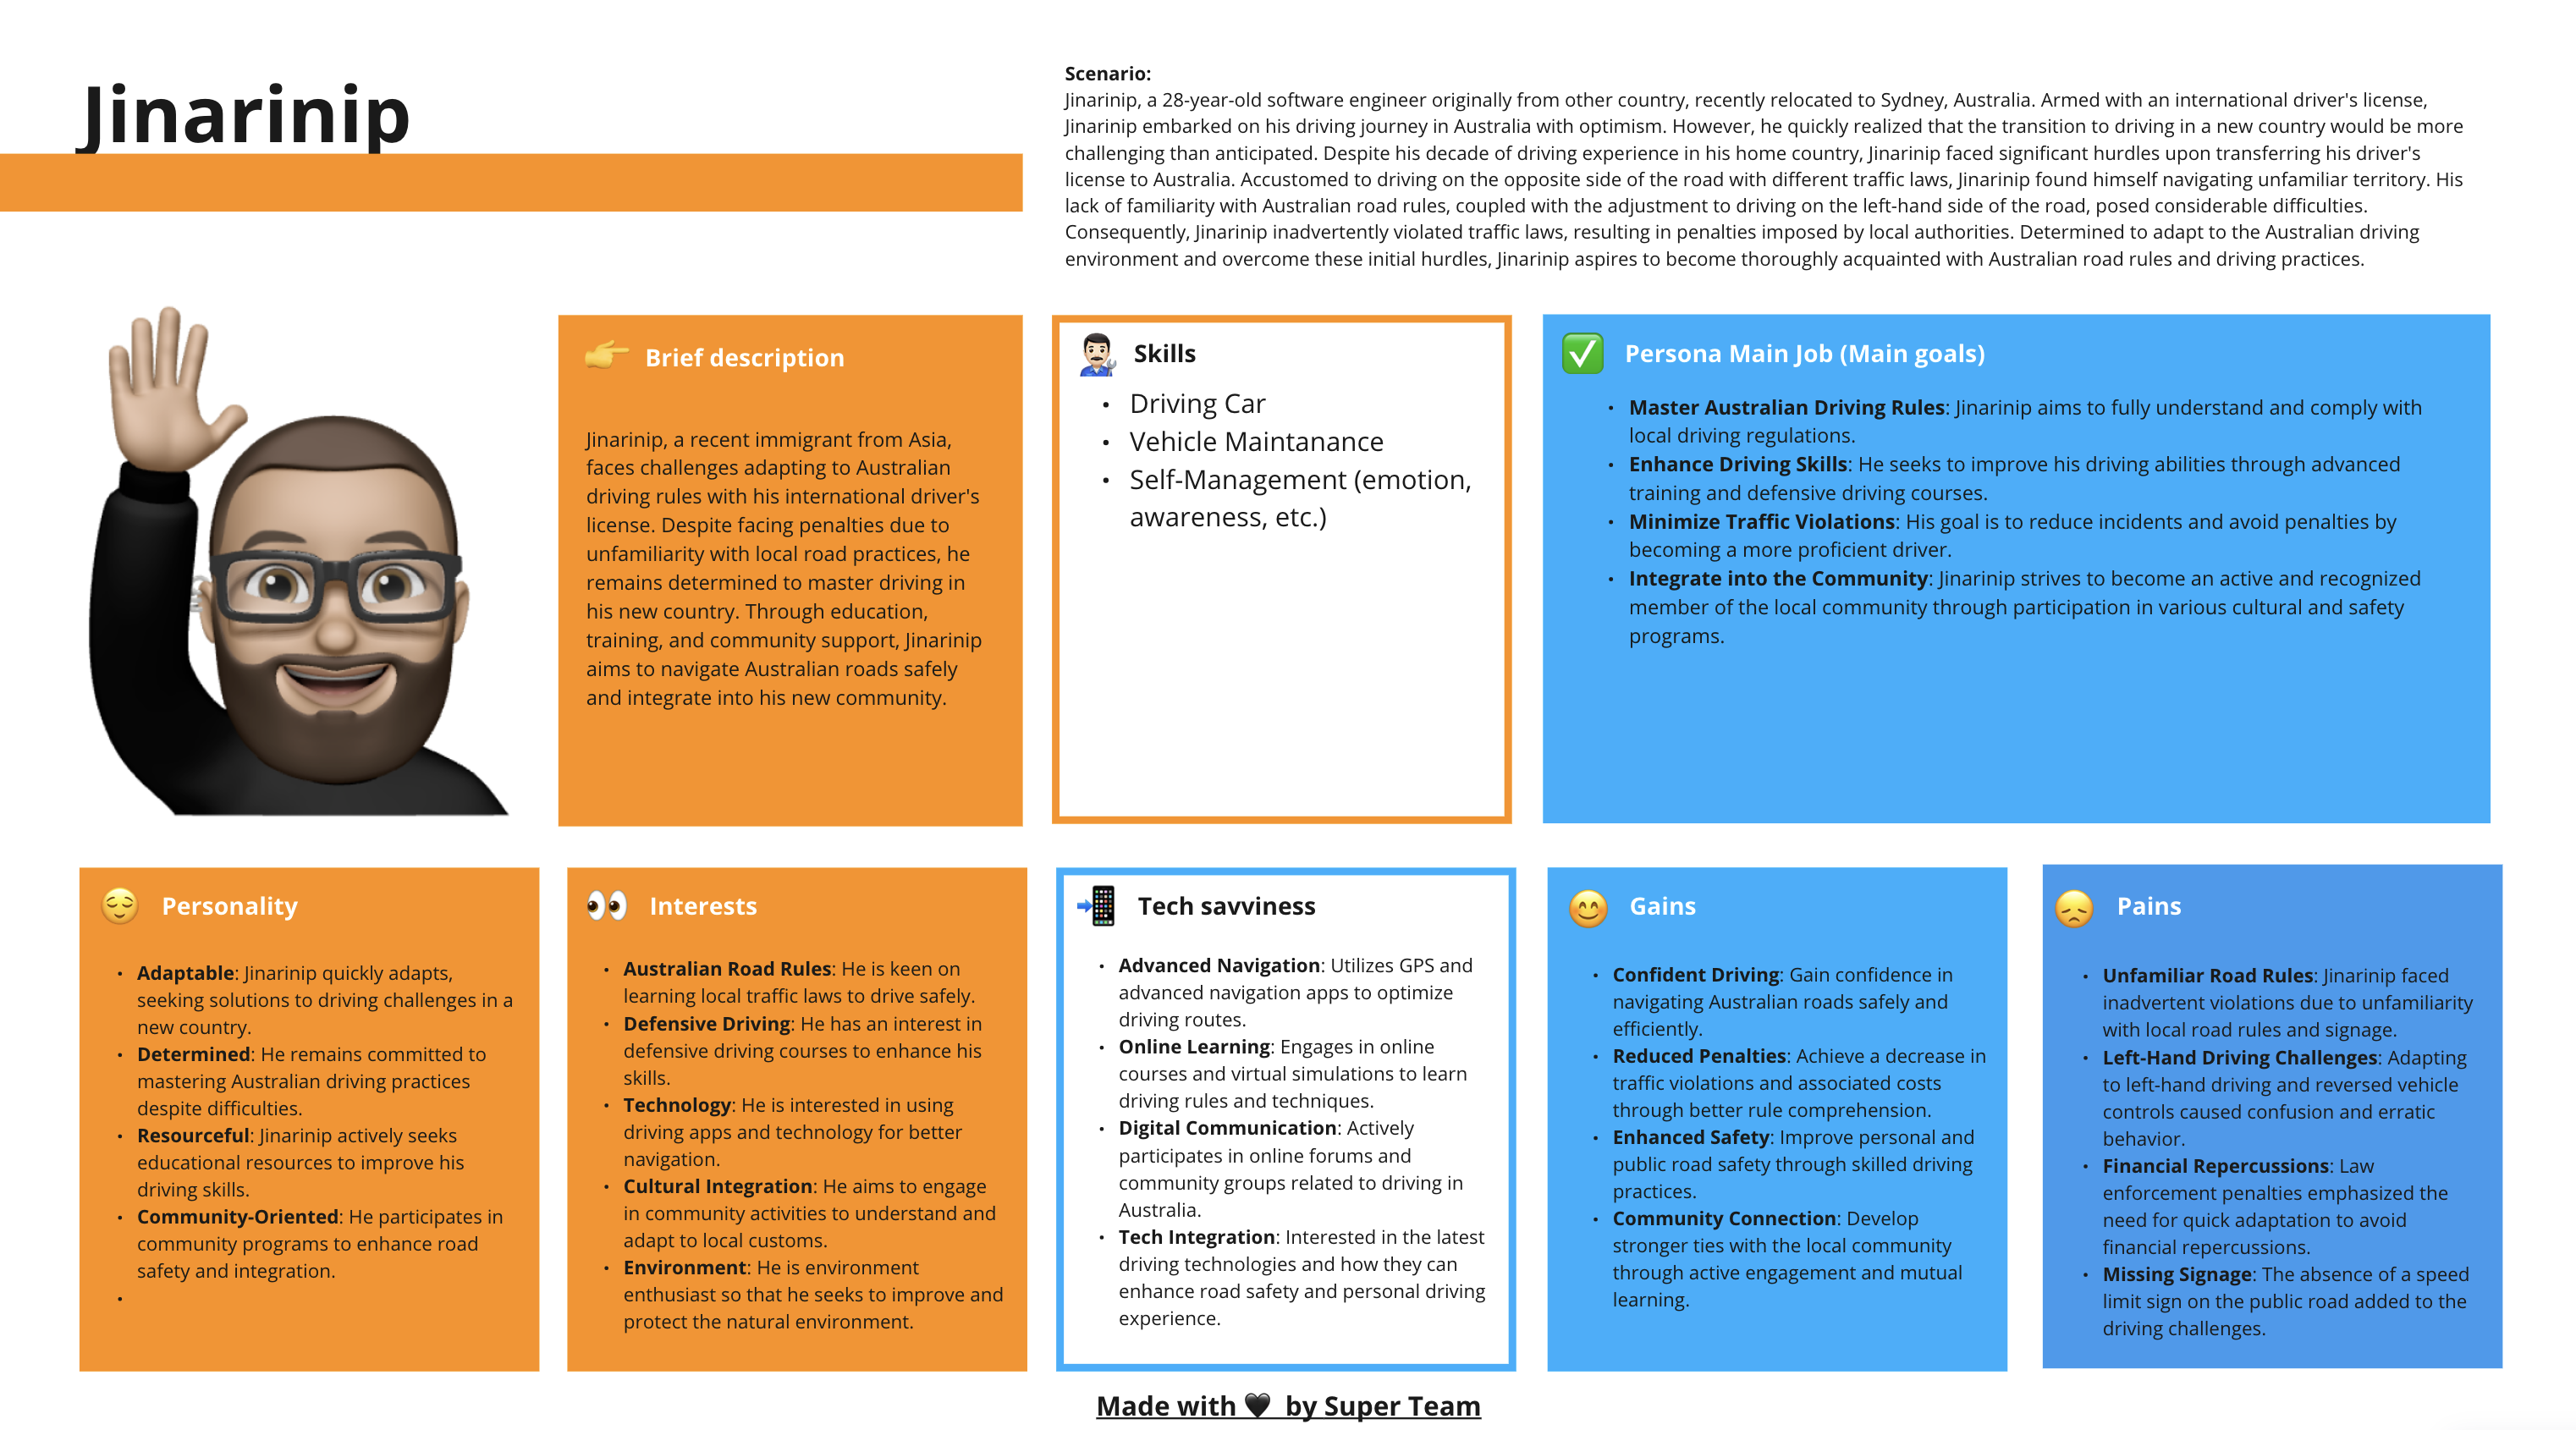
\includegraphics[width=1.0\textwidth]{images/PersonaMap.png}
    \caption{Jinarinip's Persona Map}
    \label{fig:example}
\end{figure}

\noindent The Figure 1 highlights Jinarinip's adaptation to driving in Sydney. Key components of the map include:\\

\noindent\textbf{1. Brief Description:} Jinarinip, an Asian immigrant in Sydney, is determined to master local driving regulations to fully integrate into his new community, overcoming challenges like unfamiliar road rules and potential traffic fines.\\

\noindent\textbf{2. Skills and Goals:} With skills in driving and vehicle maintenance, Jinarinip aims to comply with local driving laws and avoid traffic violations, reflecting his commitment to personal growth and community participation.\\

\noindent\textbf{3. Interests and Tech Savviness:} He actively engages with driving technology and community forums, using these platforms to enhance his driving skills and connect with others.\\

\noindent\noindent\textbf{4. Gains and Pains:} Jinarinip's main gains include increased driving confidence and stronger community connections. His pains involve navigating the complexities of new traffic regulations and handling the financial risks of potential fines.


\label{sec:Question 3}
\subsection{Persona Empathy Map Description}

\begin{figure}[h]
  \centering
  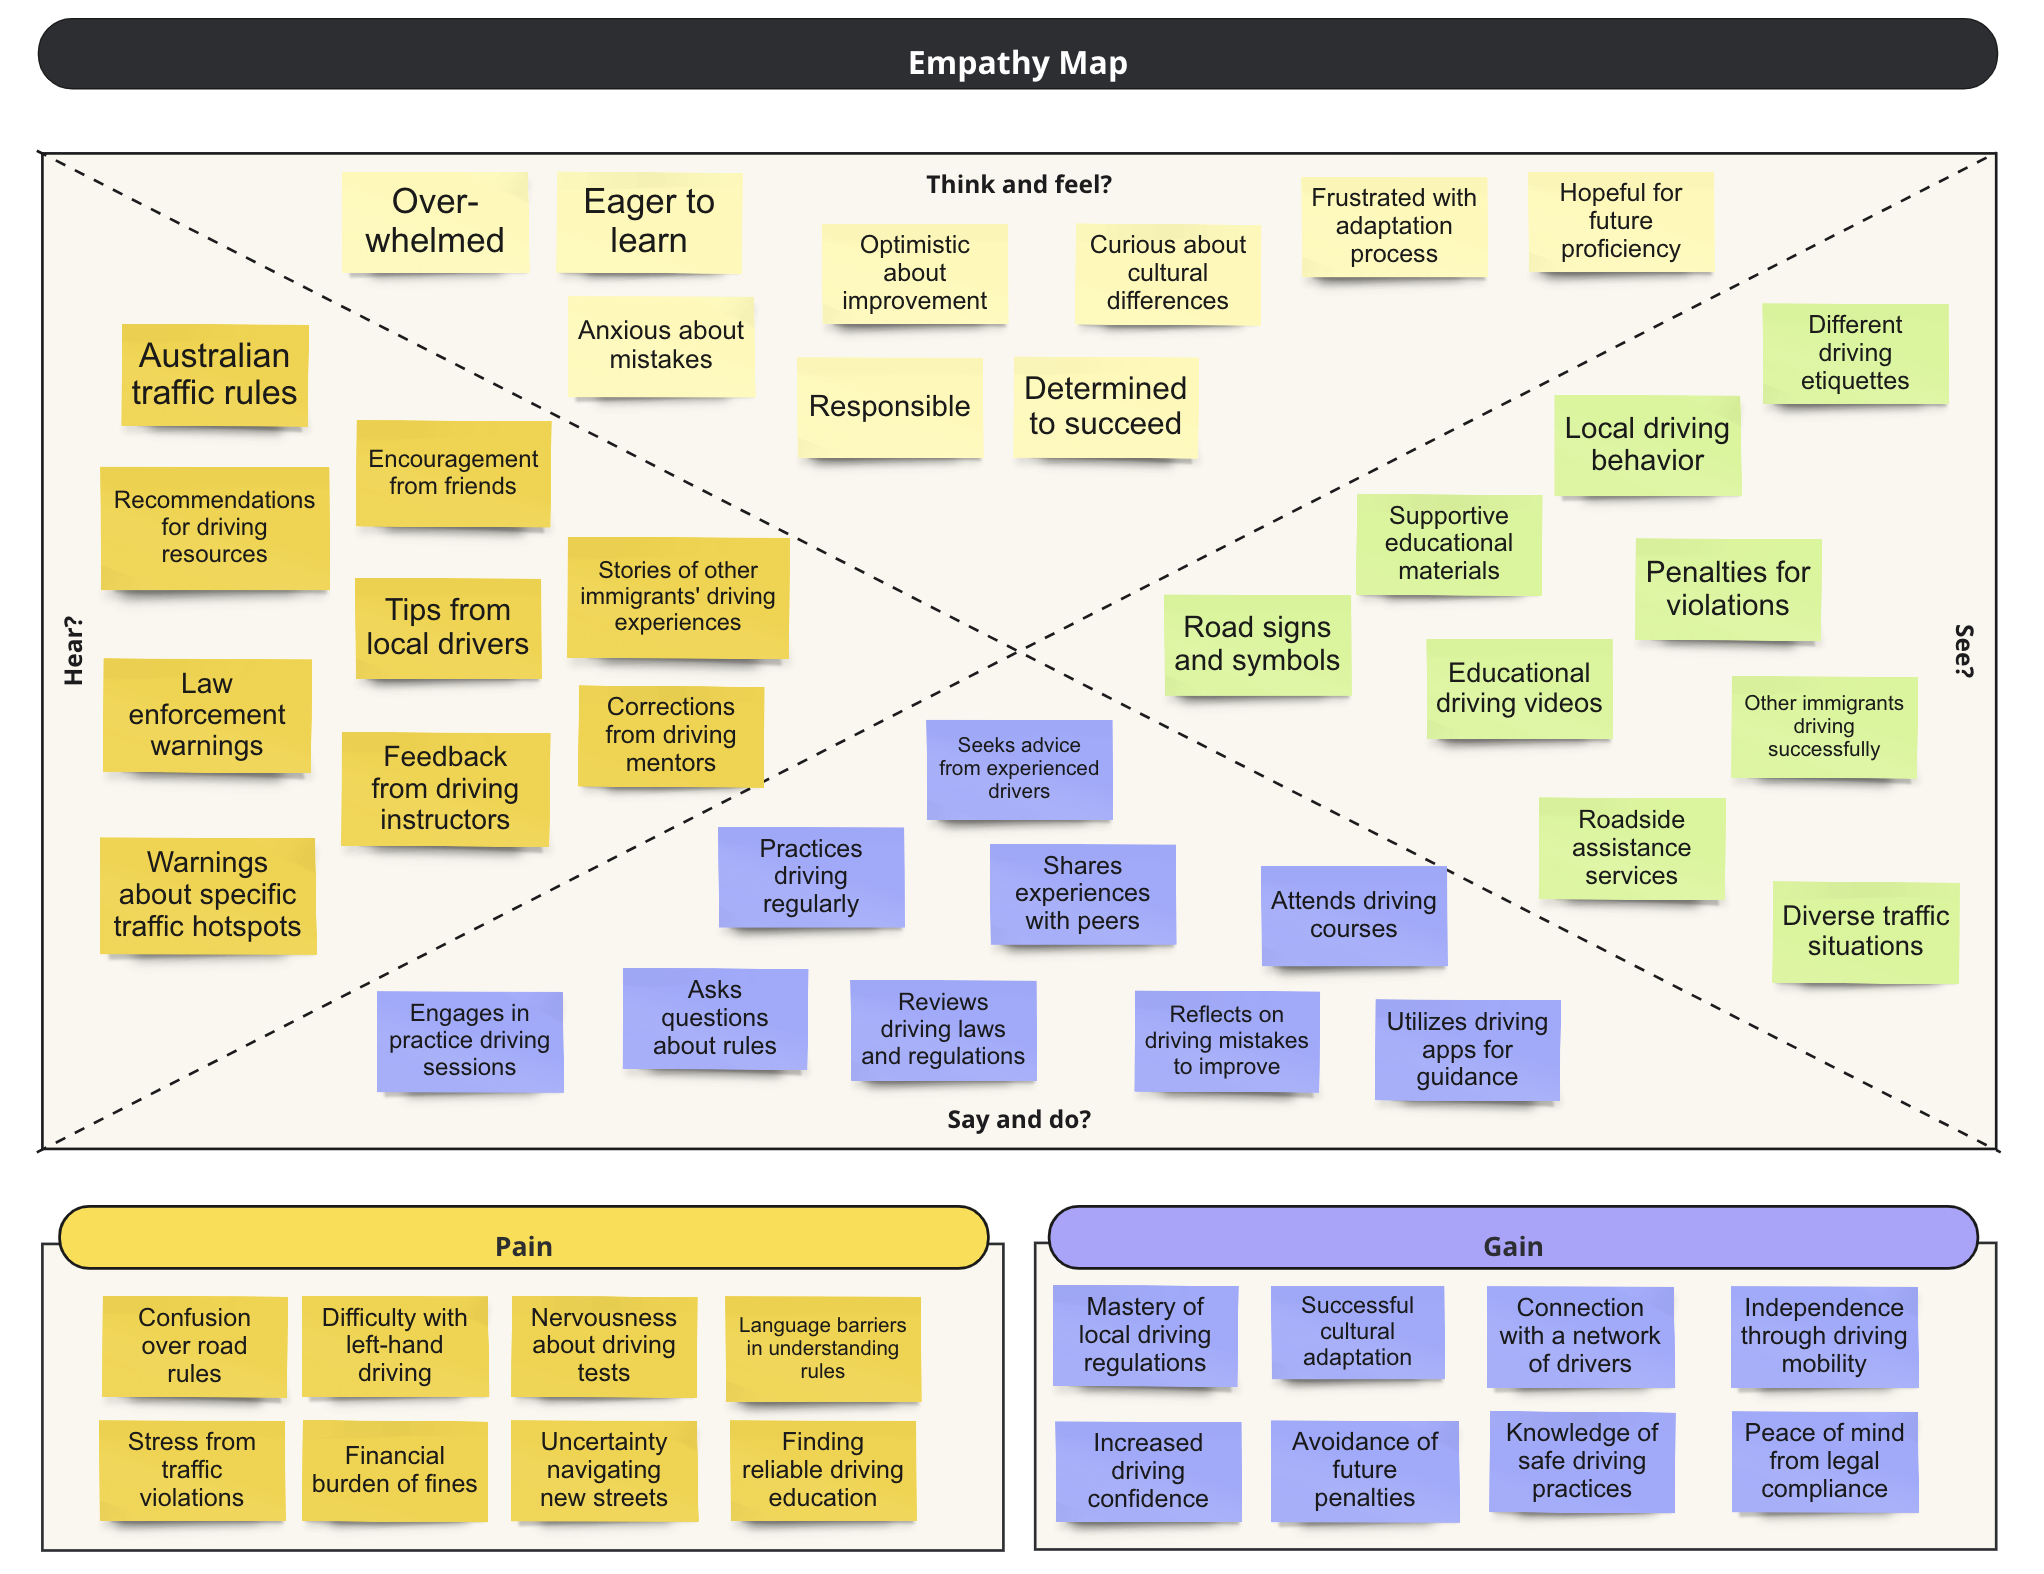
\includegraphics[width=1.0\textwidth]{images/EmpathyMap.png}
  \caption{Empathy Map for Jinarinip}
  \label{fig:empathy-map}
\end{figure}

\noindent The Figure 2 illustrates customer empathy map.

\noindent\textbf{1. Think and Feel:} Jinarinip is optimistic about mastering driving in Sydney, despite initial hurdles. His optimism is paired with a sense of responsibility and curiosity about cultural differences in driving practices, adding layers to his emotional experience as he navigates his new environment.\\

\noindent\textbf{2. Hear:} On the auditory front, Jinarinip receives a mix of encouragement and practical advice from friends and driving instructors. He also hears crucial warnings from law enforcement about traffic hotspots, which aid in his understanding of local driving norms and regulations.\\

\noindent\textbf{3. See:} Visually, Jinarinip observes road signs and symbols and watches educational driving videos. He takes note of local driving behaviors, which provide him context and insights into the practical aspects of driving in Australia.\\

\noindent\textbf{4. Say and Do:} Jinarinip actively engages in discussions with peers, asks pertinent questions about rules, and attends driving courses. He practices driving regularly and utilizes driving applications to enhance his navigation skills, demonstrating a proactive applicationroach to assimilating driving knowledge.\\

\noindent\textbf{5. Pains:} Jinarinip faces challenges such as unfamiliarity with road rules leading to penalties, difficulties with left-hand driving, and language barriers in understanding tests. These challenges cause him stress and financial strain but also motivate his pursuit of knowledge.\\

\noindent\textbf{6. Gains:} Overcoming these pains, Jinarinip gains increased driving confidence, knowledge of safe driving practices, and a deeper connection with the local community, culminating in a sense of achievement and independence.\\

\label{sec:Question 3}
\subsection{Customer Journey Map Description}


\begin{figure}[h]
  \centering
  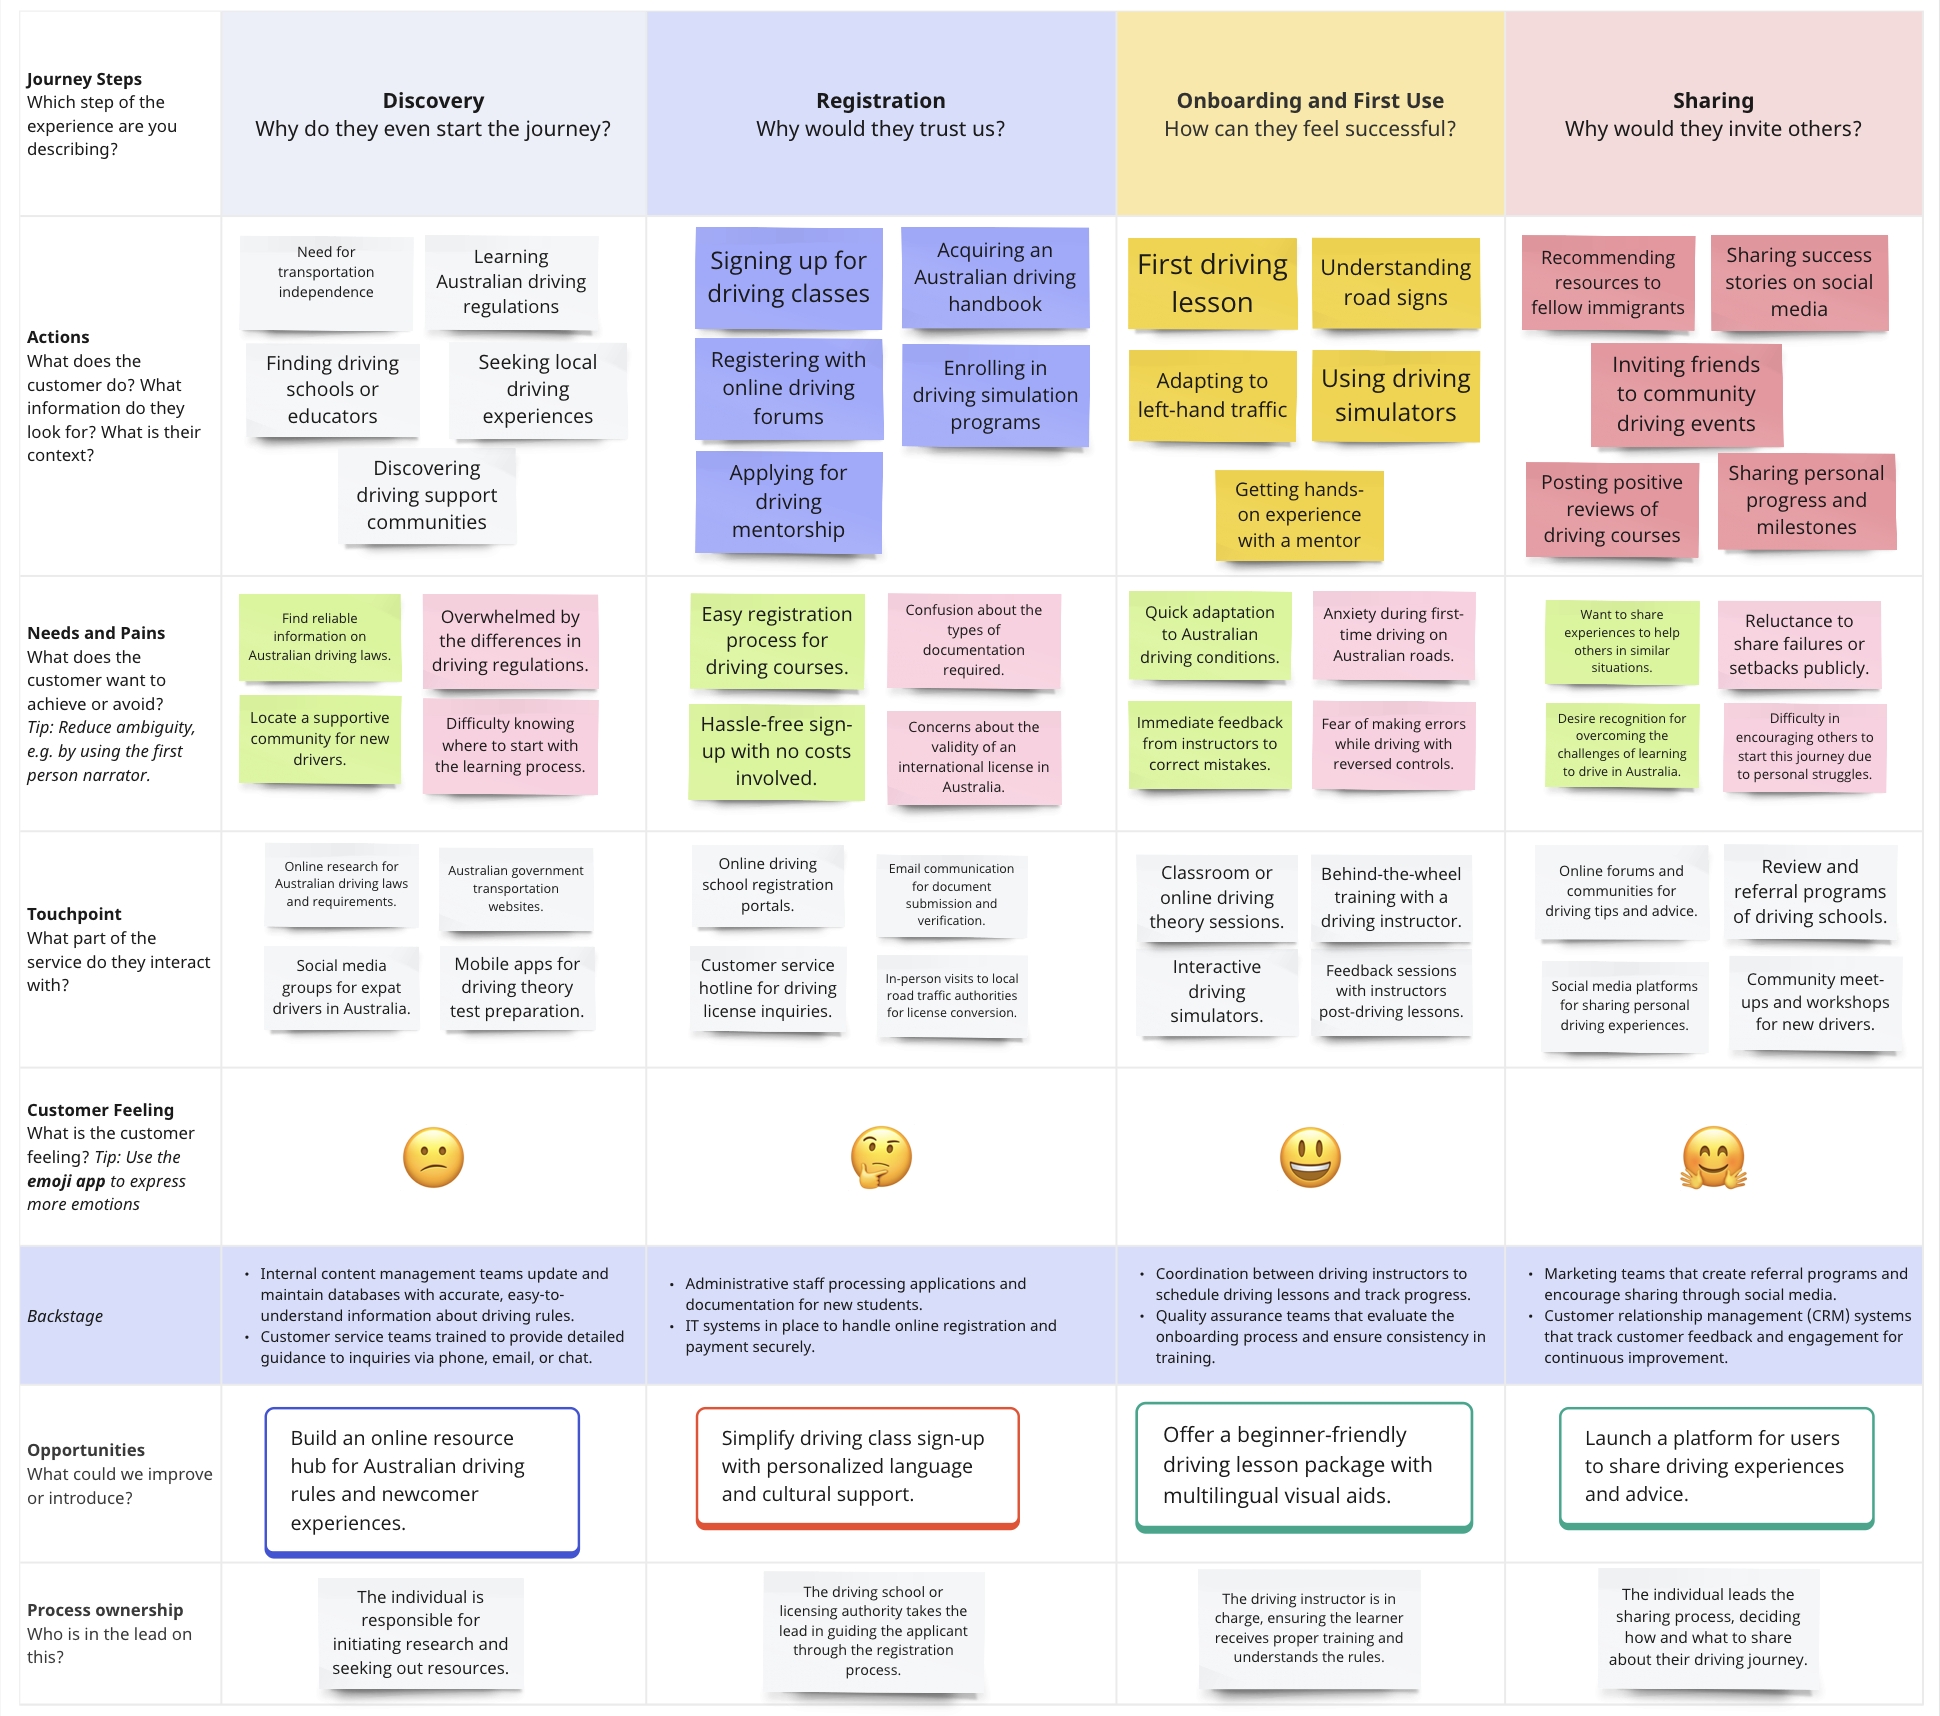
\includegraphics[width=1.0\textwidth]{images/JourneyMap.png}
  \caption{Journey Map for Jinarinip}
  \label{fig:empathy-map}
\end{figure}

\noindent\textbf{1. Discovery:} Jinarinip's journey starts with his need for transportation upon moving to Sydney. Seeking independence, he explores local driving regulations and finds driving schools and support communities that help him navigate the complexities of driving in Australia.\\

\noindent\textbf{2. Registration:} During the registration phase, Jinarinip enrolls in driving classes and applicationlies for an Australian driving handbook. Although the registration process is straightforward, he feels a mild confusion regarding the different types of documentation required, and he is concerned about the validity of his international license in Australia.
\\

\noindent\textbf{3. Onboarding and First Use:} Jinarinip's first driving lesson involves adapting to left-hand traffic and understanding local road signs through practical experience and driving simulators. Despite initial anxiety about making errors, particularly with reversed controls, the interactive lessons provide him with a reassuring hands-on experience.
\\

\noindent\textbf{4. Sharing:} Pleased with his progress and the quality of the driving lessons, Jinarinip shares his experiences on social media and recommends the courses to other immigrants. His actions reflect a desire to help others navigate similar challenges and adapt to driving in Australia.
\\

\noindent\textbf{5. Touchpoints:} Throughout his learning journey, Jinarinip engages with various aspects of the driving school, including classroom interactions, feedback from instructors post-lessons, and community forums for driving. His emotional reactions vary from nervous excitement during driving simulations to satisfaction as he gains confidence.\\

\noindent\textbf{6. Opportunities for Improvement:} The journey highlights several areas for improvement. Simplifying the class registration with personalized language support would help alleviate initial confusions. Offering beginner-friendly driving lessons that include multilingual visual aids would also enhance the learning experience for international drivers like Jinarinip. Additionally, clearer guidance on navigating local driving laws and regulations would greatly assist new drivers in becoming more confident and safe on the road\\

\noindent The Figure 3 shows that this narrative aligns closely with the journey map's stages and touchpoints, providing a structured overview of Jinarinip's experiences and the potential enhancements that could elevate his and similar users' satisfaction and safety.\\

\noindent The Figure 1, Figure 2 and Figure 3 used above were created via MIRO and are based on following references:

\begin{itemize}
    \item \cite{question_2.1}.
    \item \cite{question_2.2}.
    \item \cite{question_2.4}.    
\end{itemize}

\pagebreak

%%%%%%%%%%%%%%%%%%%%%%%%%%%%%%%%%%%%%%%%%%%%%%%%%%%%%%%%%%%%%%%%%%%%%%%%%%%%%%%%

\setcounter{page}{6}
\label{sec:Question 3}
\section{Task 3}

\subsection{Joint Value Proposition of ClearWay application }
\begin{figure}[htbp]
    \centering
    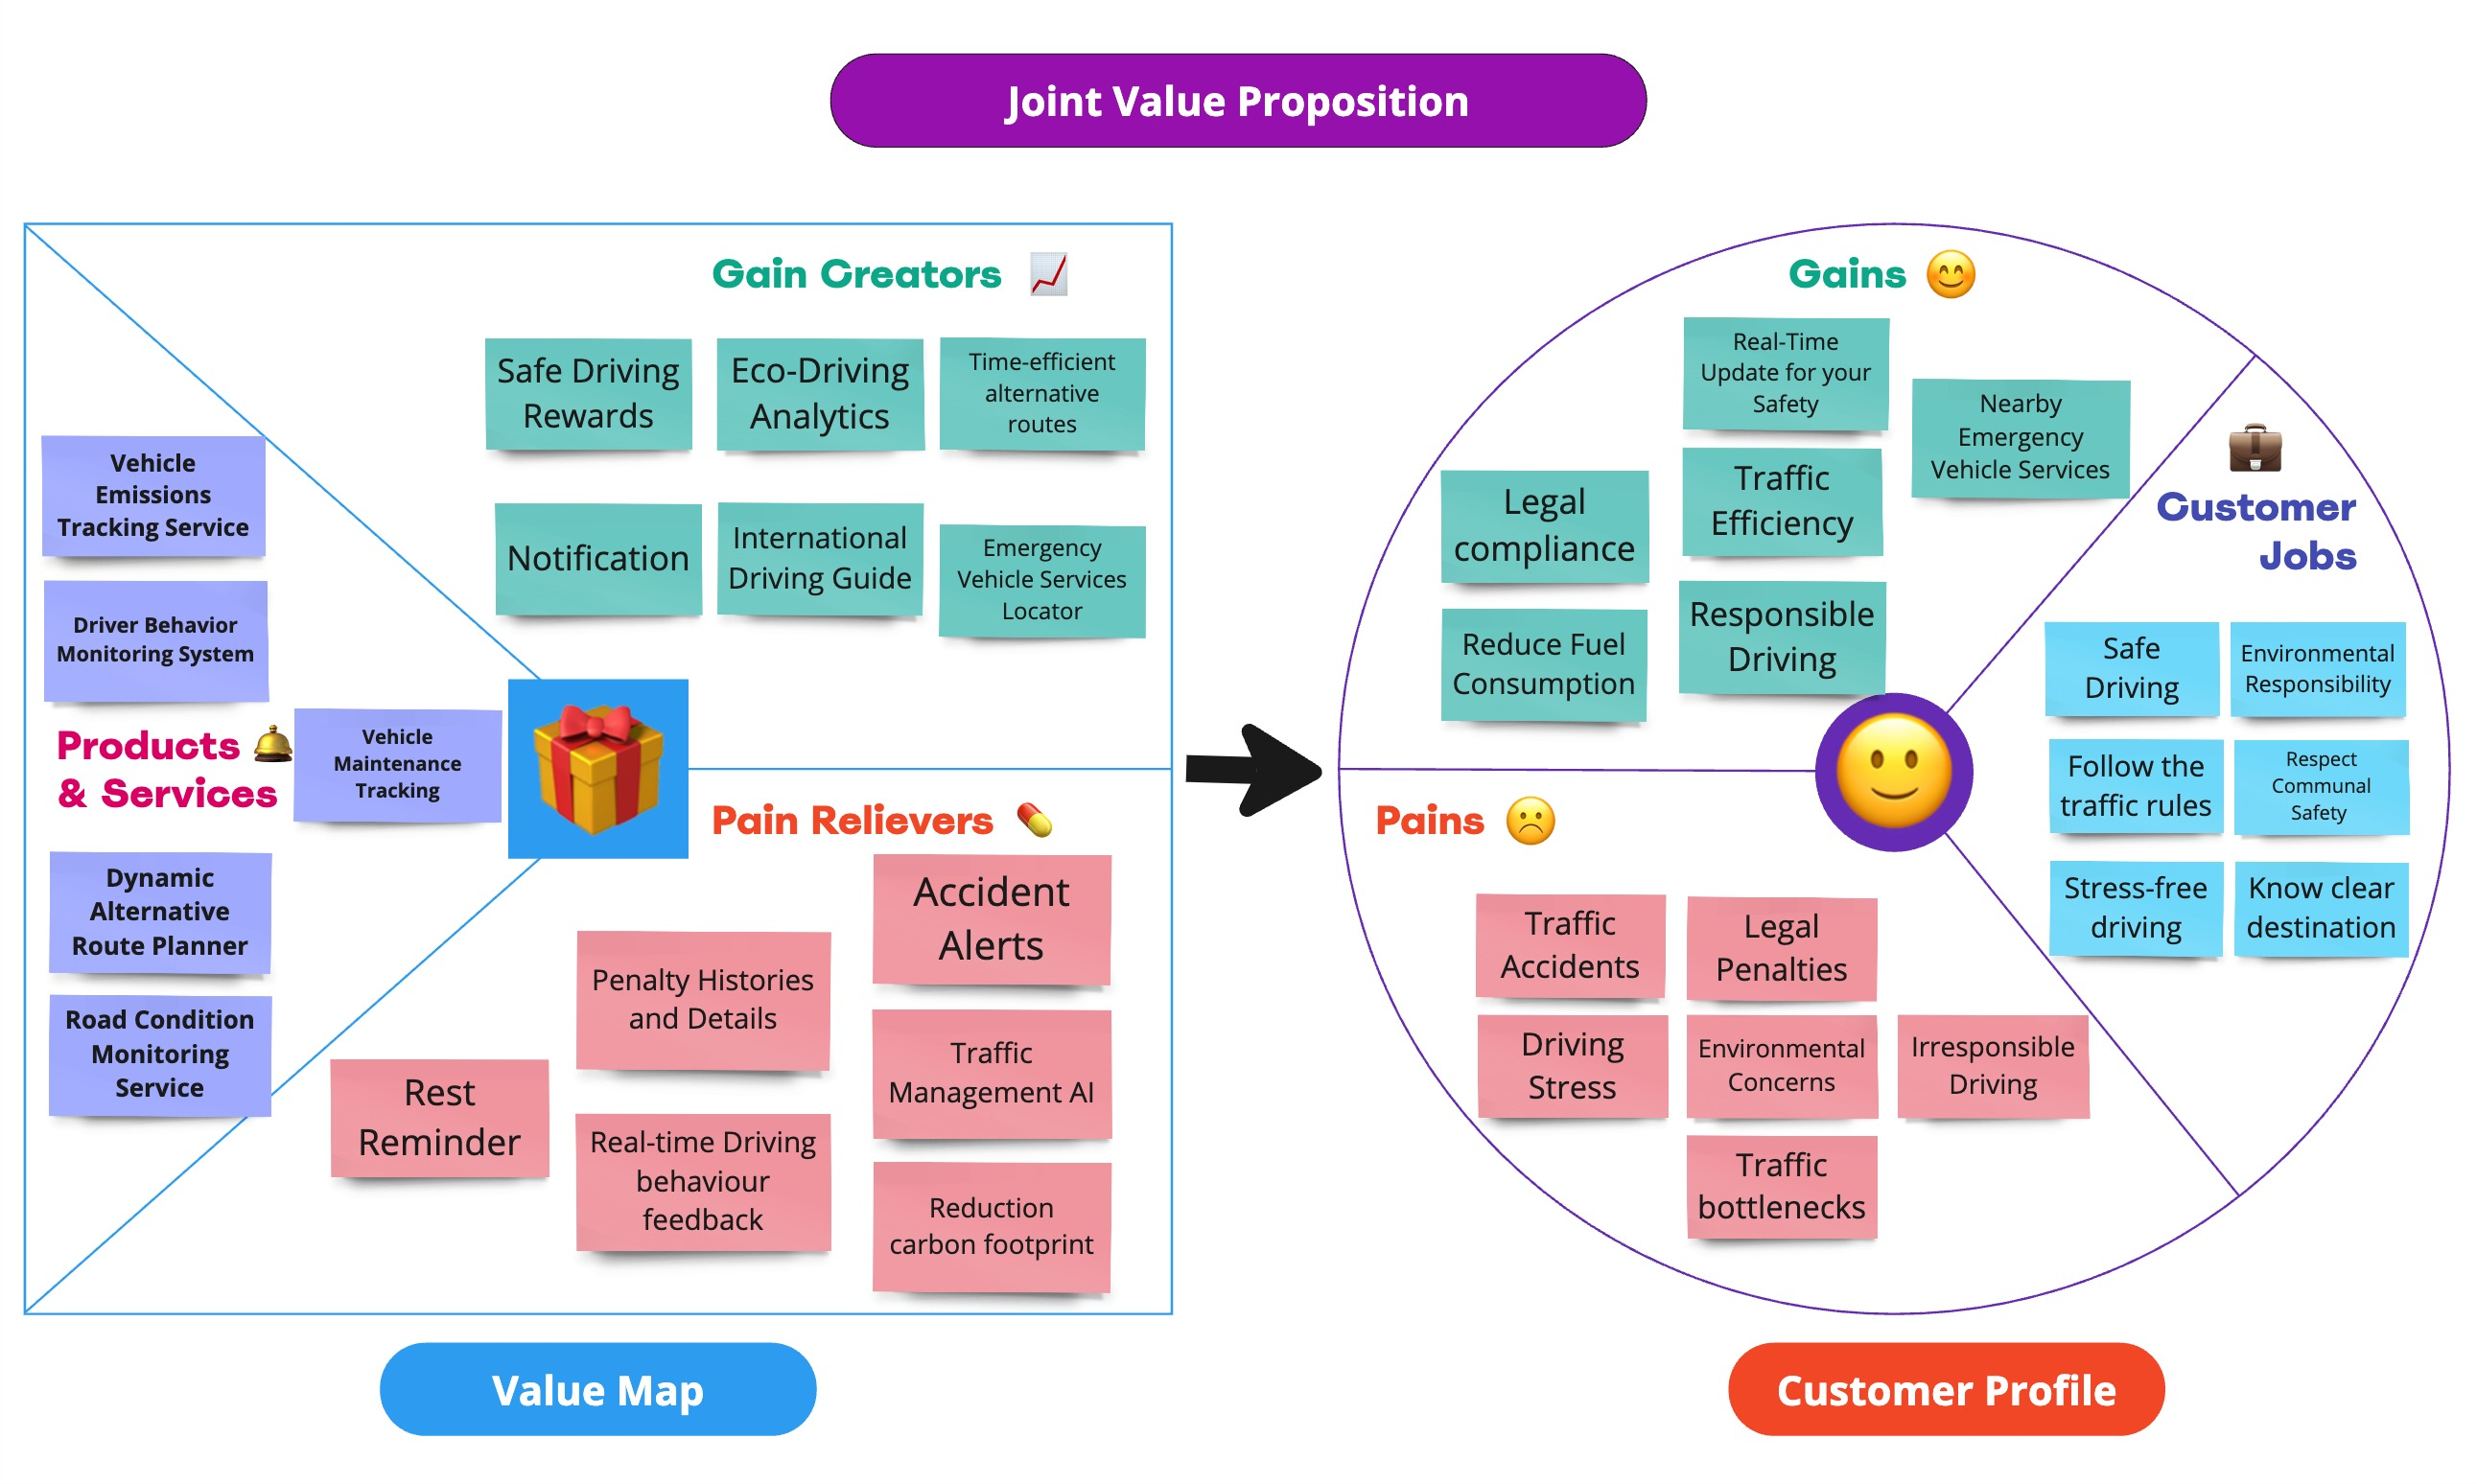
\includegraphics[width=1.0\textwidth]{images/Joint Value Proposition.jpg}
    \caption{ClearWay application Joint Value Proposition}
    \label{fig:example}
\end{figure}

\noindent\text{This Figure 4 was created using Miro and is based on \cite{Ref2.1}.}

\subsection{ClearWay application Value Proposition Overview}
\noindent \textbf{Executive Summary:}\\
\noindent Driving, an essential daily activity for millions, is ripe for transformation. ClearWay application introduces an eco-innovative applicationroach to modernize the driving experience. By seamlessly blending navigation, safety, and environmental consciousness, we offer an unparalleled mobile application tailored to the needs of the contemporary driver. Our service encapsulates not just a commitment to individual convenience but also a broader pledge towards a greener planet. \\

\noindent \textbf{Headline:} \\
\noindent Enroute to a Smarter Destination: ClearWay application’s Innovative Path to Safe and Sustainable Driving\\

\noindent \textbf{Value Proposition Description: } \\
\noindent ClearWay application is a cutting-edge mobile application that enhances the driving experience with a focus on sustainability and efficiency. Our application provides dynamic analytics to encourage eco-conscious driving and optimal route navigation, thereby reducing travel time and carbon emissions. With essential real-time data, drivers can keep their vehicles in peak condition, adhere to driving regulations, and prioritize safety. ClearWay application is dedicated to solving prevalent driving problems through smart technology, ensuring user satisfaction and contributing to environmental conservation. \\

\noindent \textbf{Detailed Services and Benefits: }\\
\noindent ClearWay application’s offerings are a testament to our commitment to driver convenience and ecological care:
\begin{itemize}
    \item \textbf{Dynamic Route Optimization:} Leveraging real-time traffic data, ClearWay application suggests the most efficient routes, saving time and fuel.
    \item \textbf{Eco-Driving Analytics:} Our sophisticated algorithms provide actionable insights on driving habits, encouraging fuel-efficient driving practices.
    \item \textbf{Driver Behavior Monitoring:} With alerts and reports on driving patterns, ClearWay application helps users adopt safer driving behaviors.
    \item \textbf{Real-Time Vehicle Maintenance Tracking:} The application notifies drivers of upcoming maintenance tasks, ensuring that vehicles run optimally and emissions stay low.
    \item \textbf{International Driving Guides:} Access comprehensive driving guides tailored to different countries, making international travel seamless and stress-free.
\end{itemize}

\noindent \textbf{Pain Relievers:} \\
\noindent ClearWay application understands the typical pains of driving and offers robust solutions:
\begin{itemize}
    \item \textbf{Accident Alerts:} By providing timely warnings about potential road hazards, we reduce the risk of accidents.
    \item \textbf{Traffic Management AI:} Our advanced AI system helps drivers navigate through traffic jams, offering alternatives to avoid bottlenecks.
    \item \textbf{Rest Reminders:} To combat driver fatigue, our application reminds users to take necessary breaks, enhancing road safety.
    \item \textbf{Feedback on Driving Patterns:} Instant feedback on driving habits allows for immediate improvements, ensuring a safer drive.
\end{itemize}

\noindent \textbf{Gain Creators:} \\
\noindent Our users gain more than just a smooth drive; they earn rewards and peace of mind:
\begin{itemize}
    \item \textbf{Safe Driving Rewards:} ClearWay application incentivizes safe driving practices with rewards, reinforcing positive behavior.
    \item \textbf{Time-Efficient Alternative Routes:} We guarantee the most efficient routes, saving users time for the things that matter.
    \item \textbf{Emergency Vehicle Services Locator:} Quick access to nearby emergency services ensures help is always at hand.
\end{itemize}

\noindent \textbf{Customer Profile Addressed:}\\
\noindent ClearWay application targets the core activities and needs of our users:
\begin{itemize}
    \item \textbf{Safe Driving:} Our primary focus is to enhance the safety of our users and their families on the road.
    \item \textbf{Compliance with Traffic Laws:} ClearWay application ensures users are updated with the latest traffic regulations, promoting legal compliance.
    \item \textbf{Stress-Free Navigation:} By providing clear and easy-to-follow directions, we remove the stress from driving.
    \item \textbf{Environmental Responsibility:} We empower drivers to make eco-friendly choices, aligning with global sustainability goals.
\end{itemize}

 

\noindent \textbf{Pains and Gains Addressed:} \\
\noindent We confront the unpleasant aspects of driving while amplifying the benefits: 
\begin{itemize}
    \item \textbf{Pains:} Traffic accidents, legal penalties, environmental concerns, and the stress of driving are all addressed with our comprehensive set of features.
    \item \textbf{Gains:} Users enjoy the perks of up-to-date safety information, efficient route planning, and an overall enhanced driving experience.
\end{itemize}

\noindent \textbf{Conclusion:} \\
\noindent In conclusion, ClearWay application stands at the forefront of driving innovation. Our meticulously crafted application offers a holistic solution to modern-day driving dilemmas, ensuring each journey is not only safer and more efficient but also kinder to our planet. As we move forward, ClearWay application will continue to drive progress, delivering an unmatched value proposition for our users and the world they inhabit. \\




\pagebreak

%%%%%%%%%%%%%%%%%%%%%%%%%%%%%%%%%%%%%%%%%%%%%%%%%%%%%%%%%%%%%%%%%%%%%%%%%%%%%%%%

\setcounter{page}{9}
\label{sec:Question 4}
\section{Task 4}

\subsection{Two-Level Lotus Blossom Diagram of ClearWay application}
\begin{figure}[htbp]
    \centering
    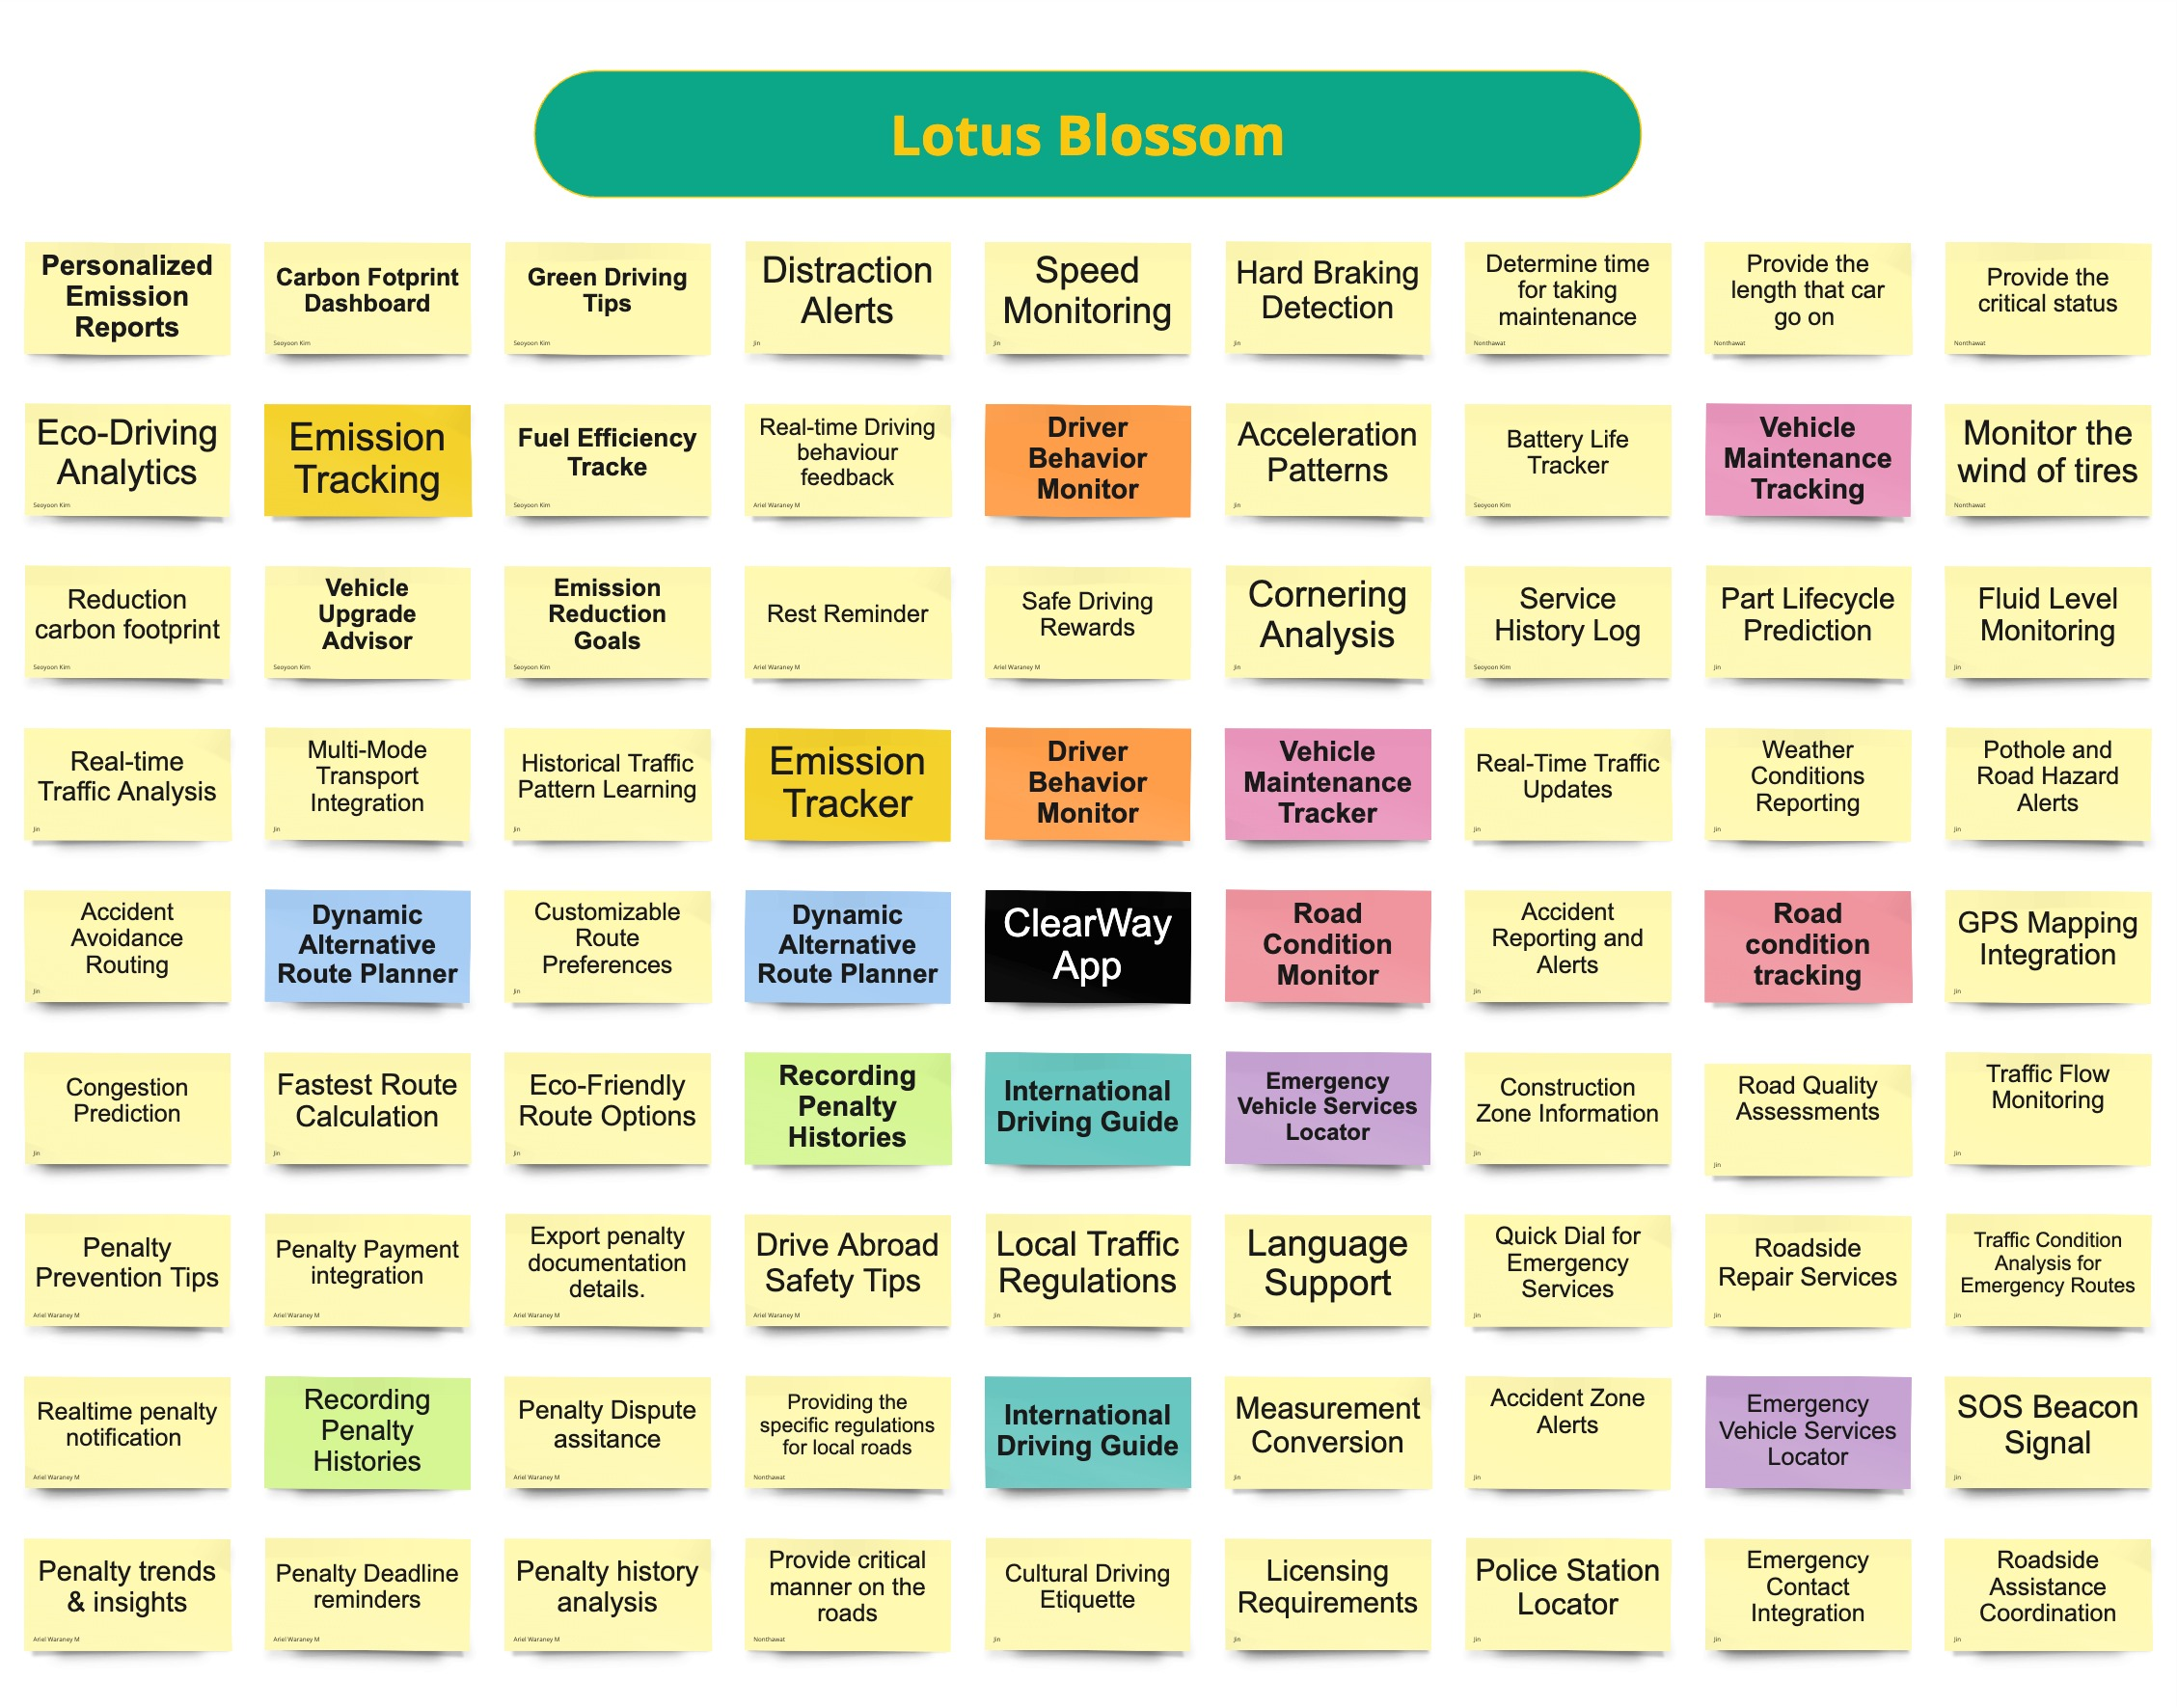
\includegraphics[width=1\textwidth]{images/Lotus Blossom.jpg}
    \caption{ClearWay application Lotus Blossom Diagram}
    \label{fig:example}
\end{figure}

This Figure 5 was created using Miro and is based on:
\begin{itemize}
    \item \cite{Ref3.1}.
    \item \cite{Ref3.2}.  
\end{itemize}

\pagebreak

%%%%%%%%%%%%%%%%%%%%%%%%%%%%%%%%%%%%%%%%%%%%%%%%%%%%%%%%%%%%%%%%%%%%%%%%%%%%%%%%

\setcounter{page}{10}
\label{sec:Question 5}
\section{Task 5}

\subsection{Revenue Model of ClearWay application}
\noindent \textbf{Freemium model:} \\
\noindent It has been used to gain a tremendous amount of acquisition as a customer base and take advantage of networking from acquisition \citep{task_5.1}. We provide essential basic features that improve their experiences and offer outstanding subscription features like monitoring road conditions, vehicle maintenance tracking, and recording penalties. We aim to create a long-lifetime customer base that can generate revenue flow for our business in subsequent years. Moreover, getting customers' data is our second priority. Sufficient data creates opportunities to identify customer needs so that we can add more attractive features to our application that will increase the subscription rate. More importantly, these activities strengthen business value, which generates revenue streams.\\

\noindent \textbf{Advertisements:} \\
\noindent As a result of our strong business value, the reliability of our application attracts various business partners. According to Eslabra, smartphone owners spend approximately 4-5 hours daily on applications \citep{task_5.2}. From this fact, we have integrated in-application advertisements and offered them to every partner, big or small, such as a local store, bank, convenience store, or service provider. Partners can rent a space on our application, whether banner, pop-up or short video, to promote their services and increase customer engagement. However, the prices are different based on the popularity of each location. In addition, we offered a bid for the best locations so that partners who give the highest offer will get it. \\

\noindent \textbf{Commission Base and revenue sharing model:} \\
\noindent This model is determined to be cost-effective for influencing customers to interact with our services \citep{task_5.3}. Strong Business Value provides collaboration opportunities with partnerships like insurance companies, emergency services, roadside assistance, and government institutes. This generates a sustainable revenue stream by receiving customer commissions from interacting with partners' services. For instance, our business receives commissions when customers call for roadside assistance. On top of that, our application receives sales percentages from services that customers pay for, which builds a strong revenue stream for us. \\


\pagebreak

%%%%%%%%%%%%%%%%%%%%%%%%%%%%%%%%%%%%%%%%%%%%%%%%%%%%%%%%%%%%%%%%%%%%%%%%%%%%%%%%

\setcounter{page}{11}
\label{sec:Question 6}
\section{Task 6}

\subsection{Low-Fidelity Prototype of ClearWay application}
\noindent Based on our joint value proposition, we developed a low-fidelity prototype using Figma, classified as a digital prototype for its flexibility and efficiency \citep{question_6.1}, to showcase the five main features of our Clearway's products and services. Figure 6 illustrates the user journey, beginning with discovering and downloading the application. Users are greeted by a welcome page offering login options for registered users and sign-up options for new users. Both login and registration processes are straightforward and free of charge. Upon completing these steps, users can access the home page, which includes tab bar menus at the bottom of the screen.\\
\begin{figure}[h]
    \centering
    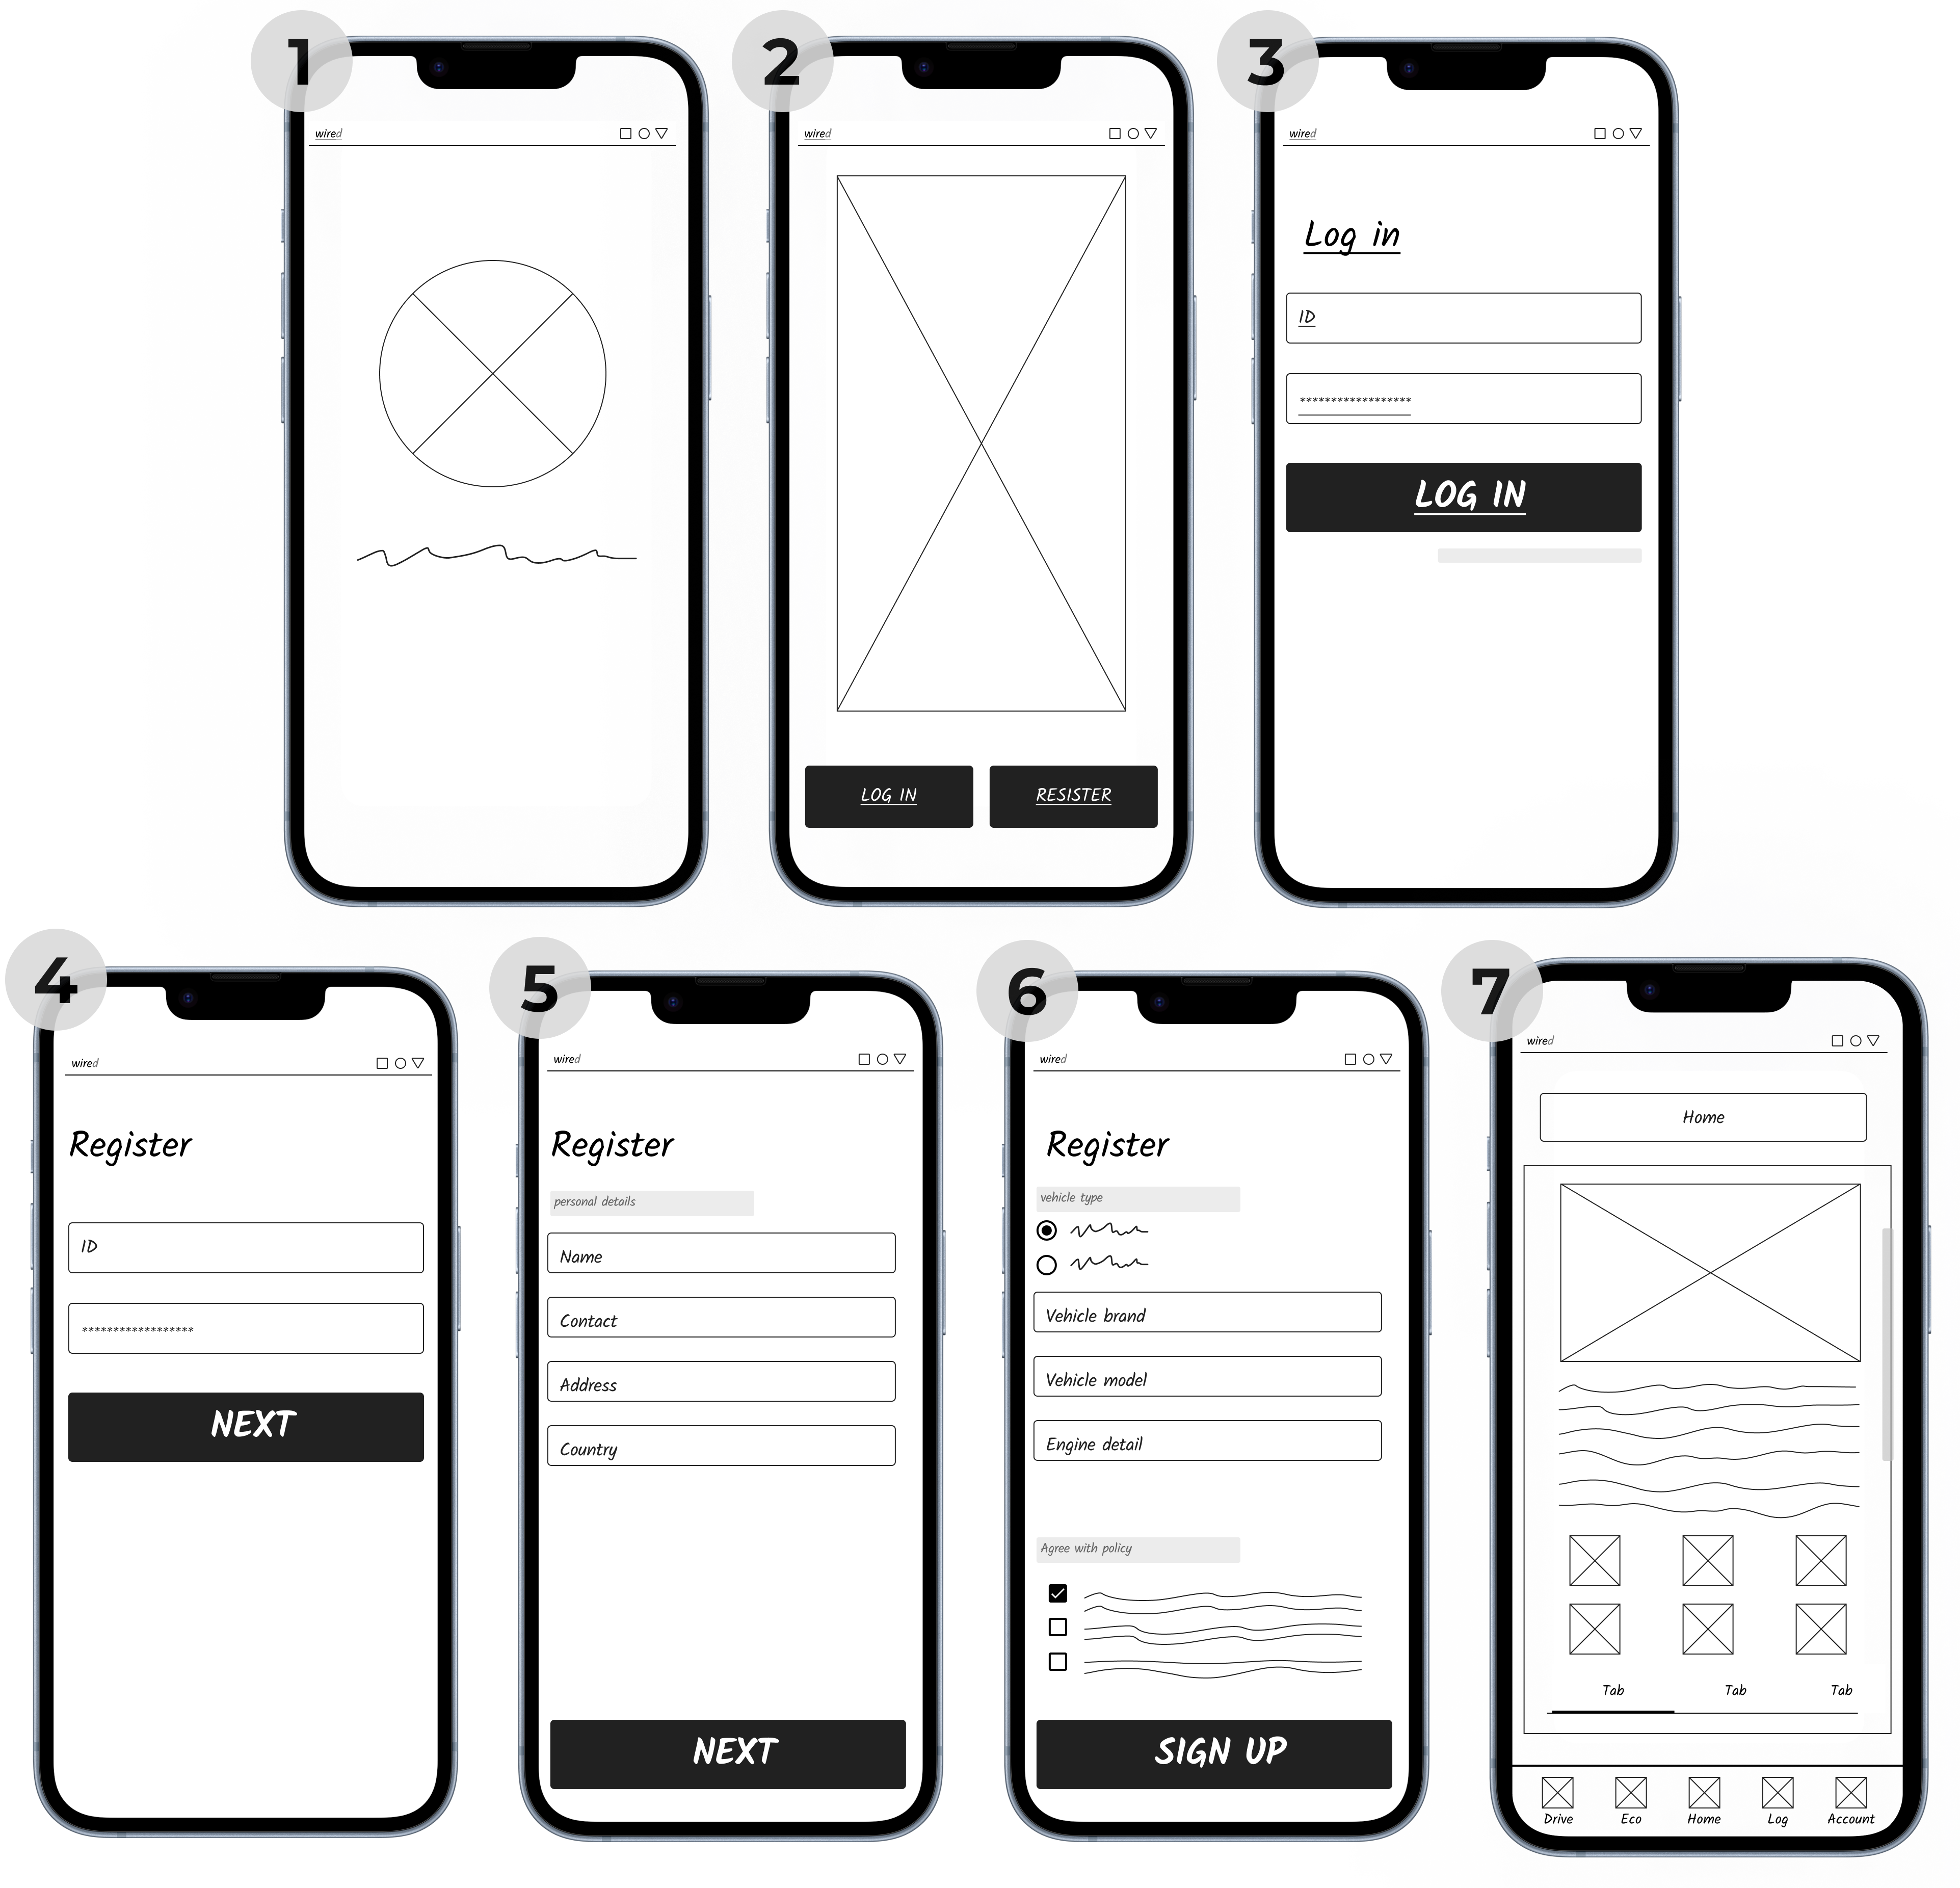
\includegraphics[width=0.8
    \textwidth]{images/Prototype Figures/Prototype Figure 1.png}
    \caption{Login \& Register Process}
    \label{fig:example}
\end{figure}



\noindent From the home screen, users can view summaries and overviews based on their driving records. As a driving electronic-assistant, our application provides enhanced guides and information that helps drivers in a particular country to quickly understand local driving policies and patterns, ensuring safe driving. Figure 7 shows that users can select any country from a list; for each country, the application displays important notices, including driving culture and measurement conversions (miles or kilometers). This is one of the primary, value-added features we have developed.\\
\begin{figure}[h]
    \centering
    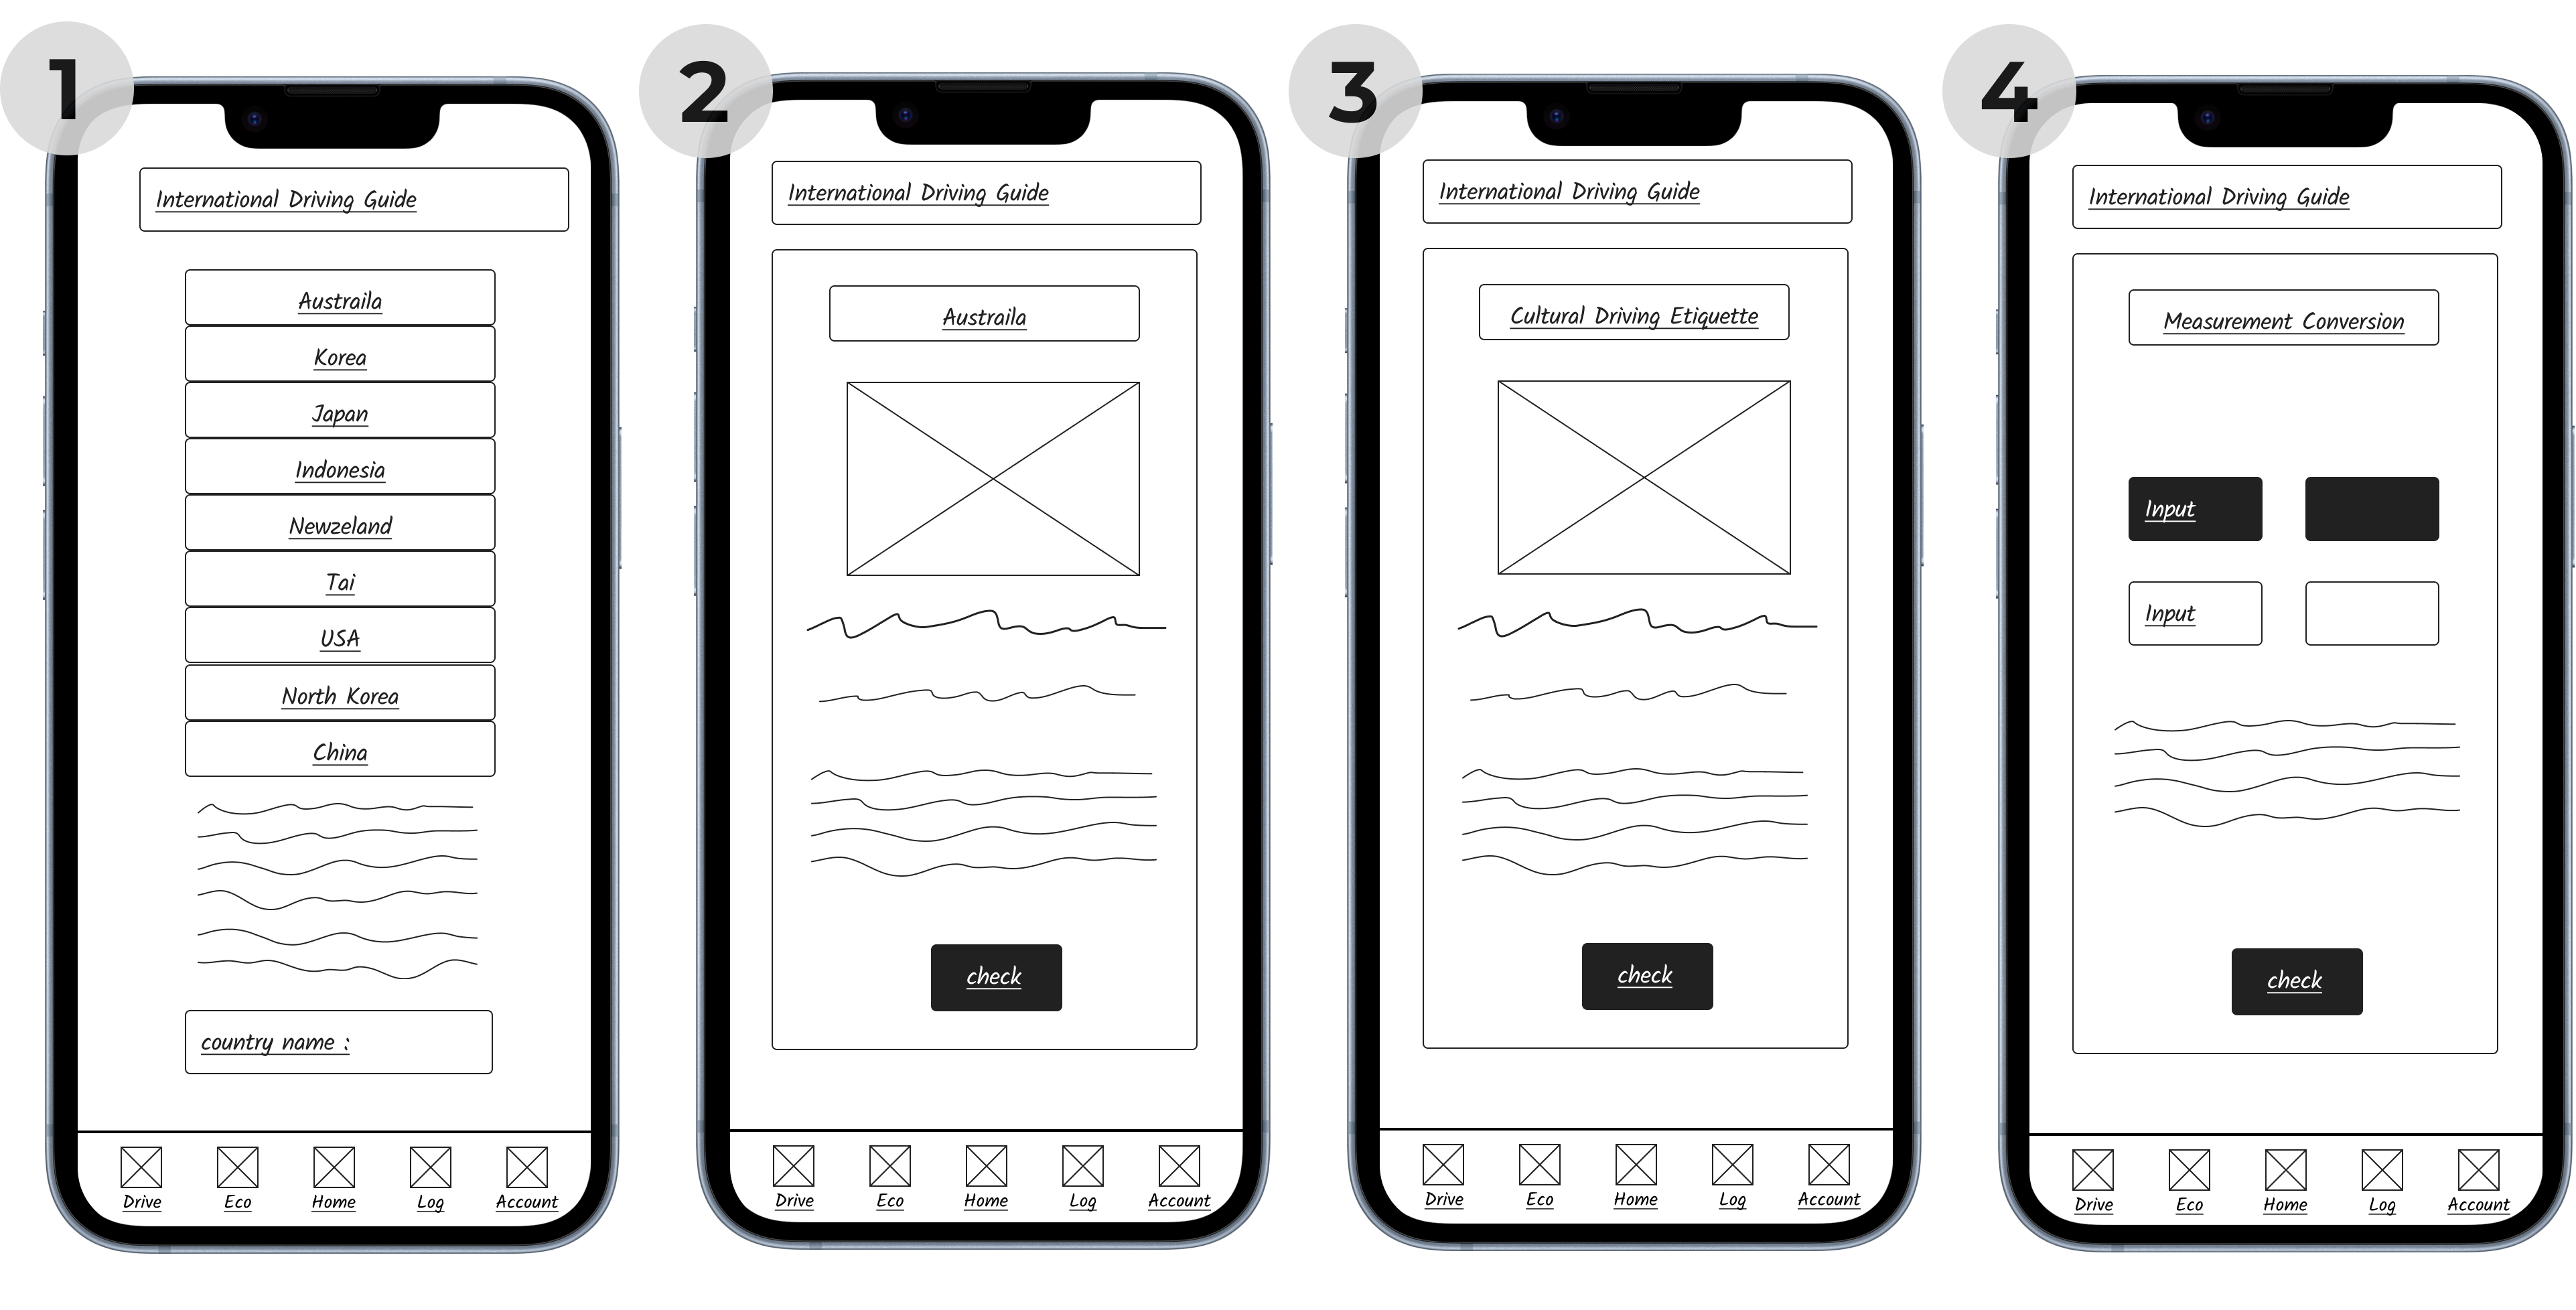
\includegraphics[width=0.8
    \textwidth]{images/Prototype Figures/Prototype Figure 2.png}
    \caption{International Driving Guide}
    \label{fig:example}
\end{figure}



\noindent Various features are accessible via the tab bar menu. Under the `Eco" menu, is the Emission Tracking to promote Eco-Driving. Figure 8 illustrates how users can monitor their carbon footprint reduction through graphs, receive vehicle upgrade advice for environmental purposes, analyze eco-driving performances, and track fuel efficiency. These tools align with user’s problem of addressing environmental concerns by promoting fuel efficiency and eco-friendly driving practices to their best.\\
\begin{figure}[h]
    \centering
    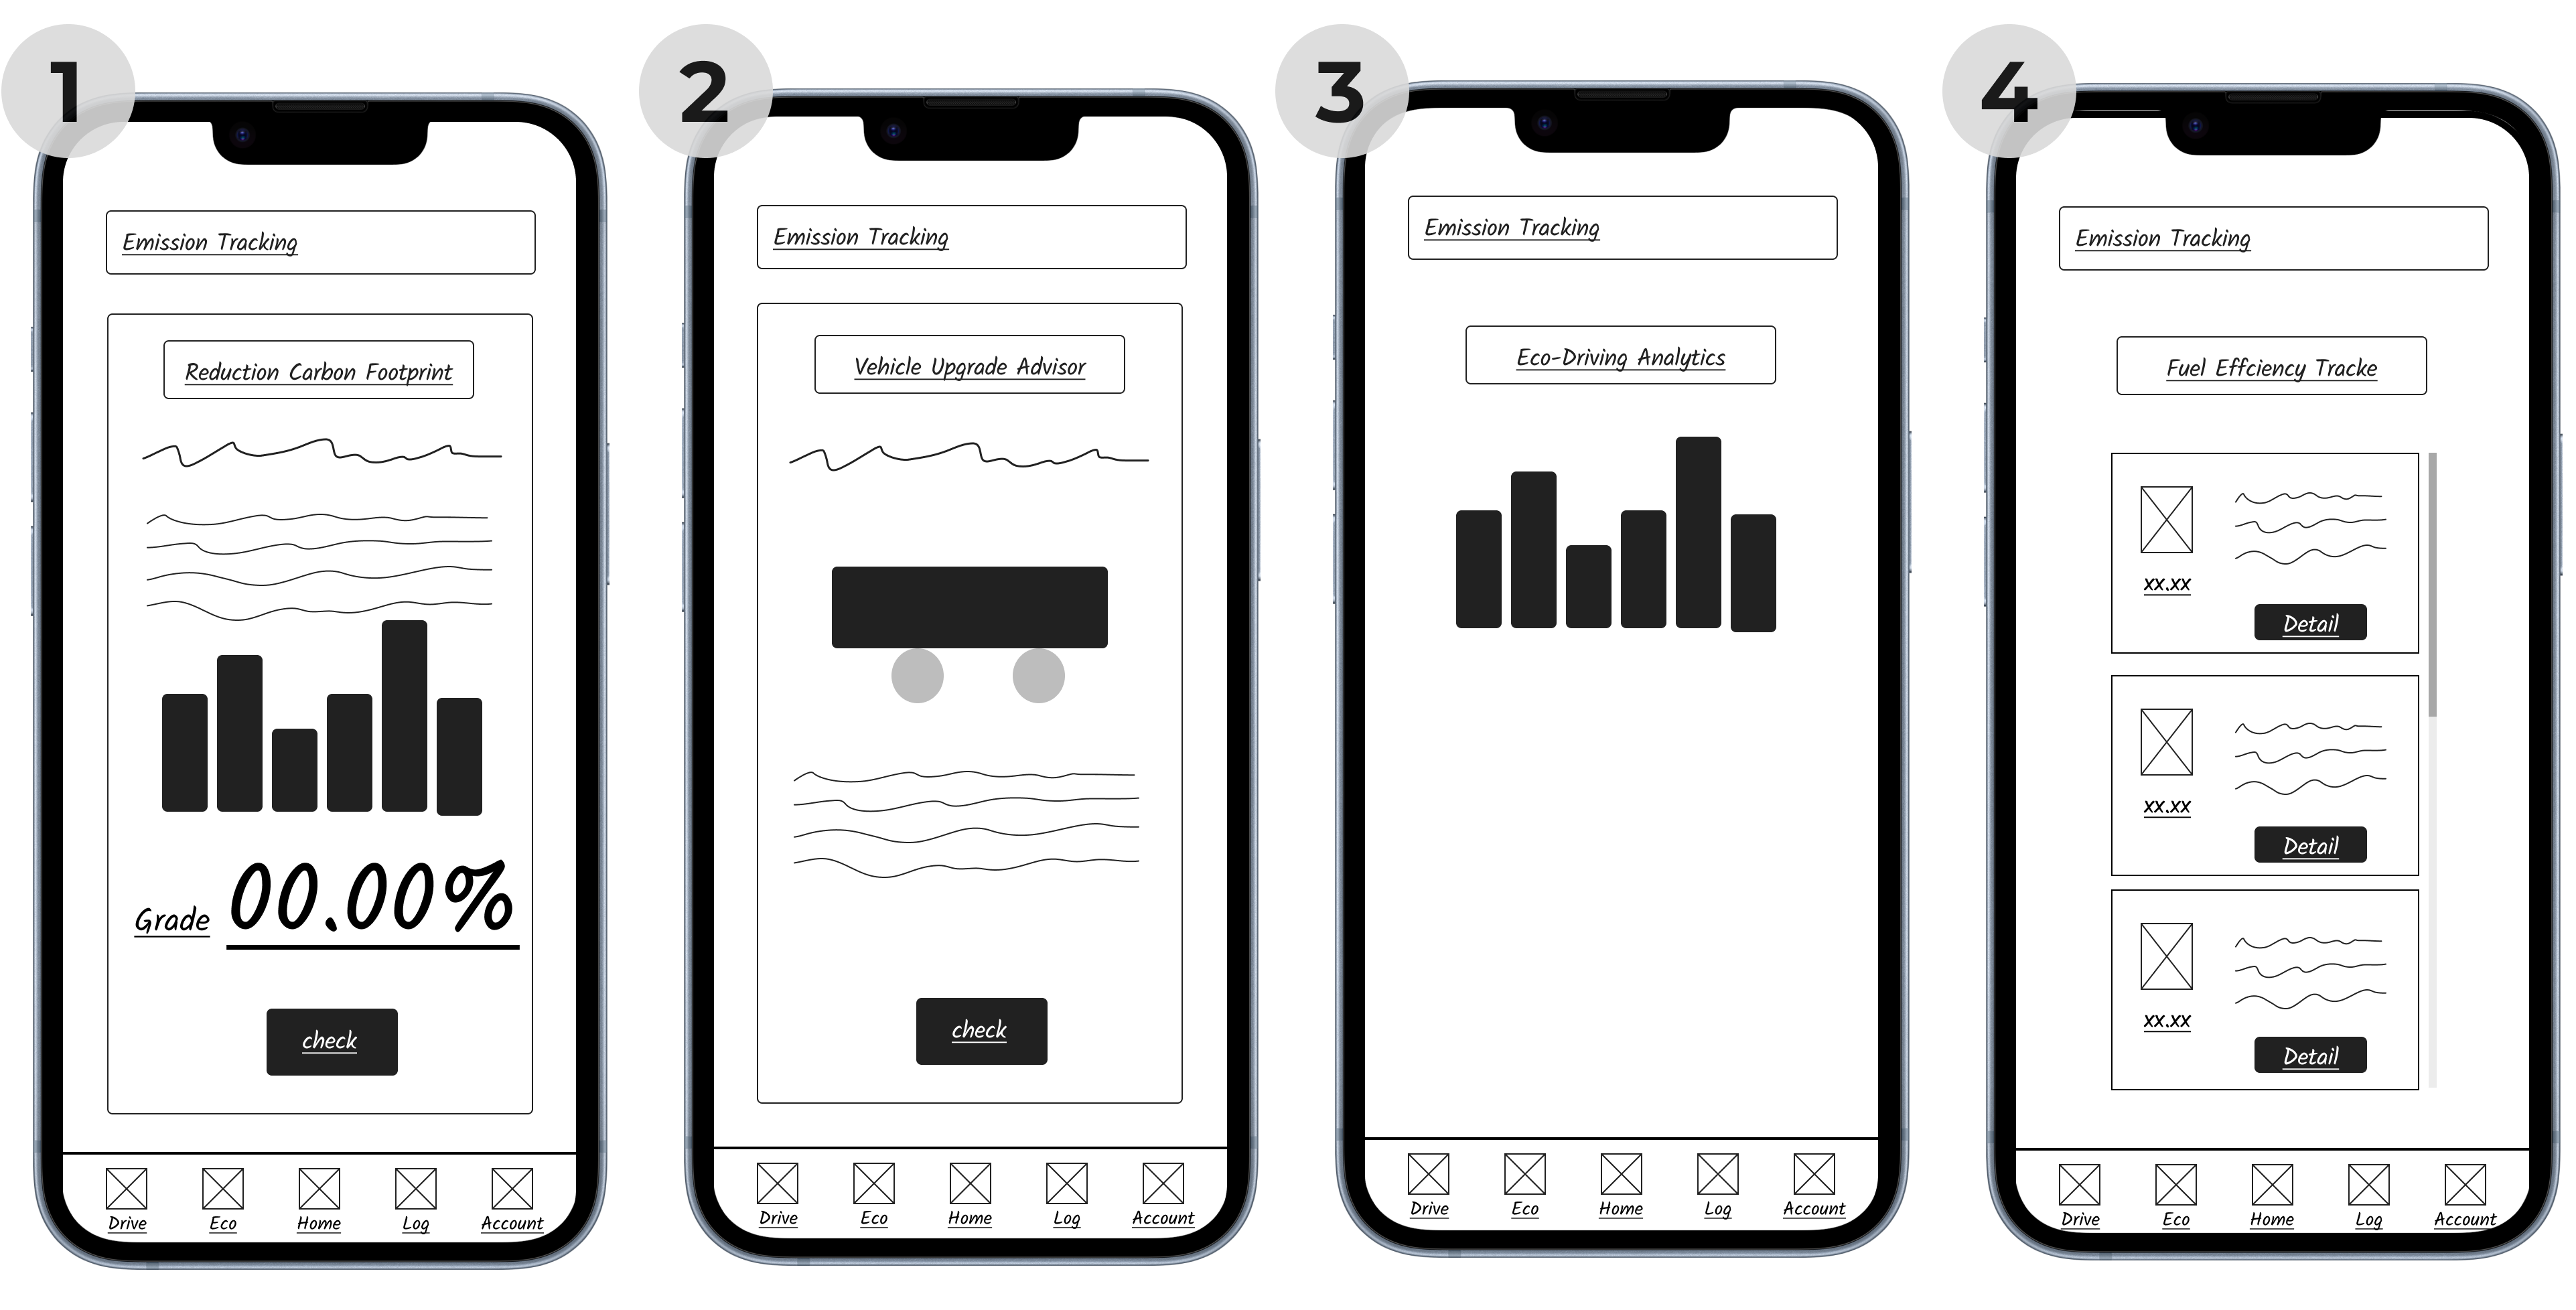
\includegraphics[width=0.8
    \textwidth]{images/Prototype Figures/Prototype Figure 3.png}
    \caption{Eco Driving Feature}
    \label{fig:example}
\end{figure}




\noindent Under the `Drive' menu, is the dynamic alternative route planner - our main feature. Figure 9 displays a map where users set their destination, and the application identifies the most efficient route from their current location. The planner is dynamic, allowing users to select their preferred route—be it the fastest, traffic-free, or other options. The application utilizes real-time traffic analysis to recognize historical patterns, traffic bottlenecks,  suggest accident avoidance routes, and predict congestion. Users can view and select route indicators from the checkbox options above the map panel.\\

\begin{figure}[h]
    \centering
    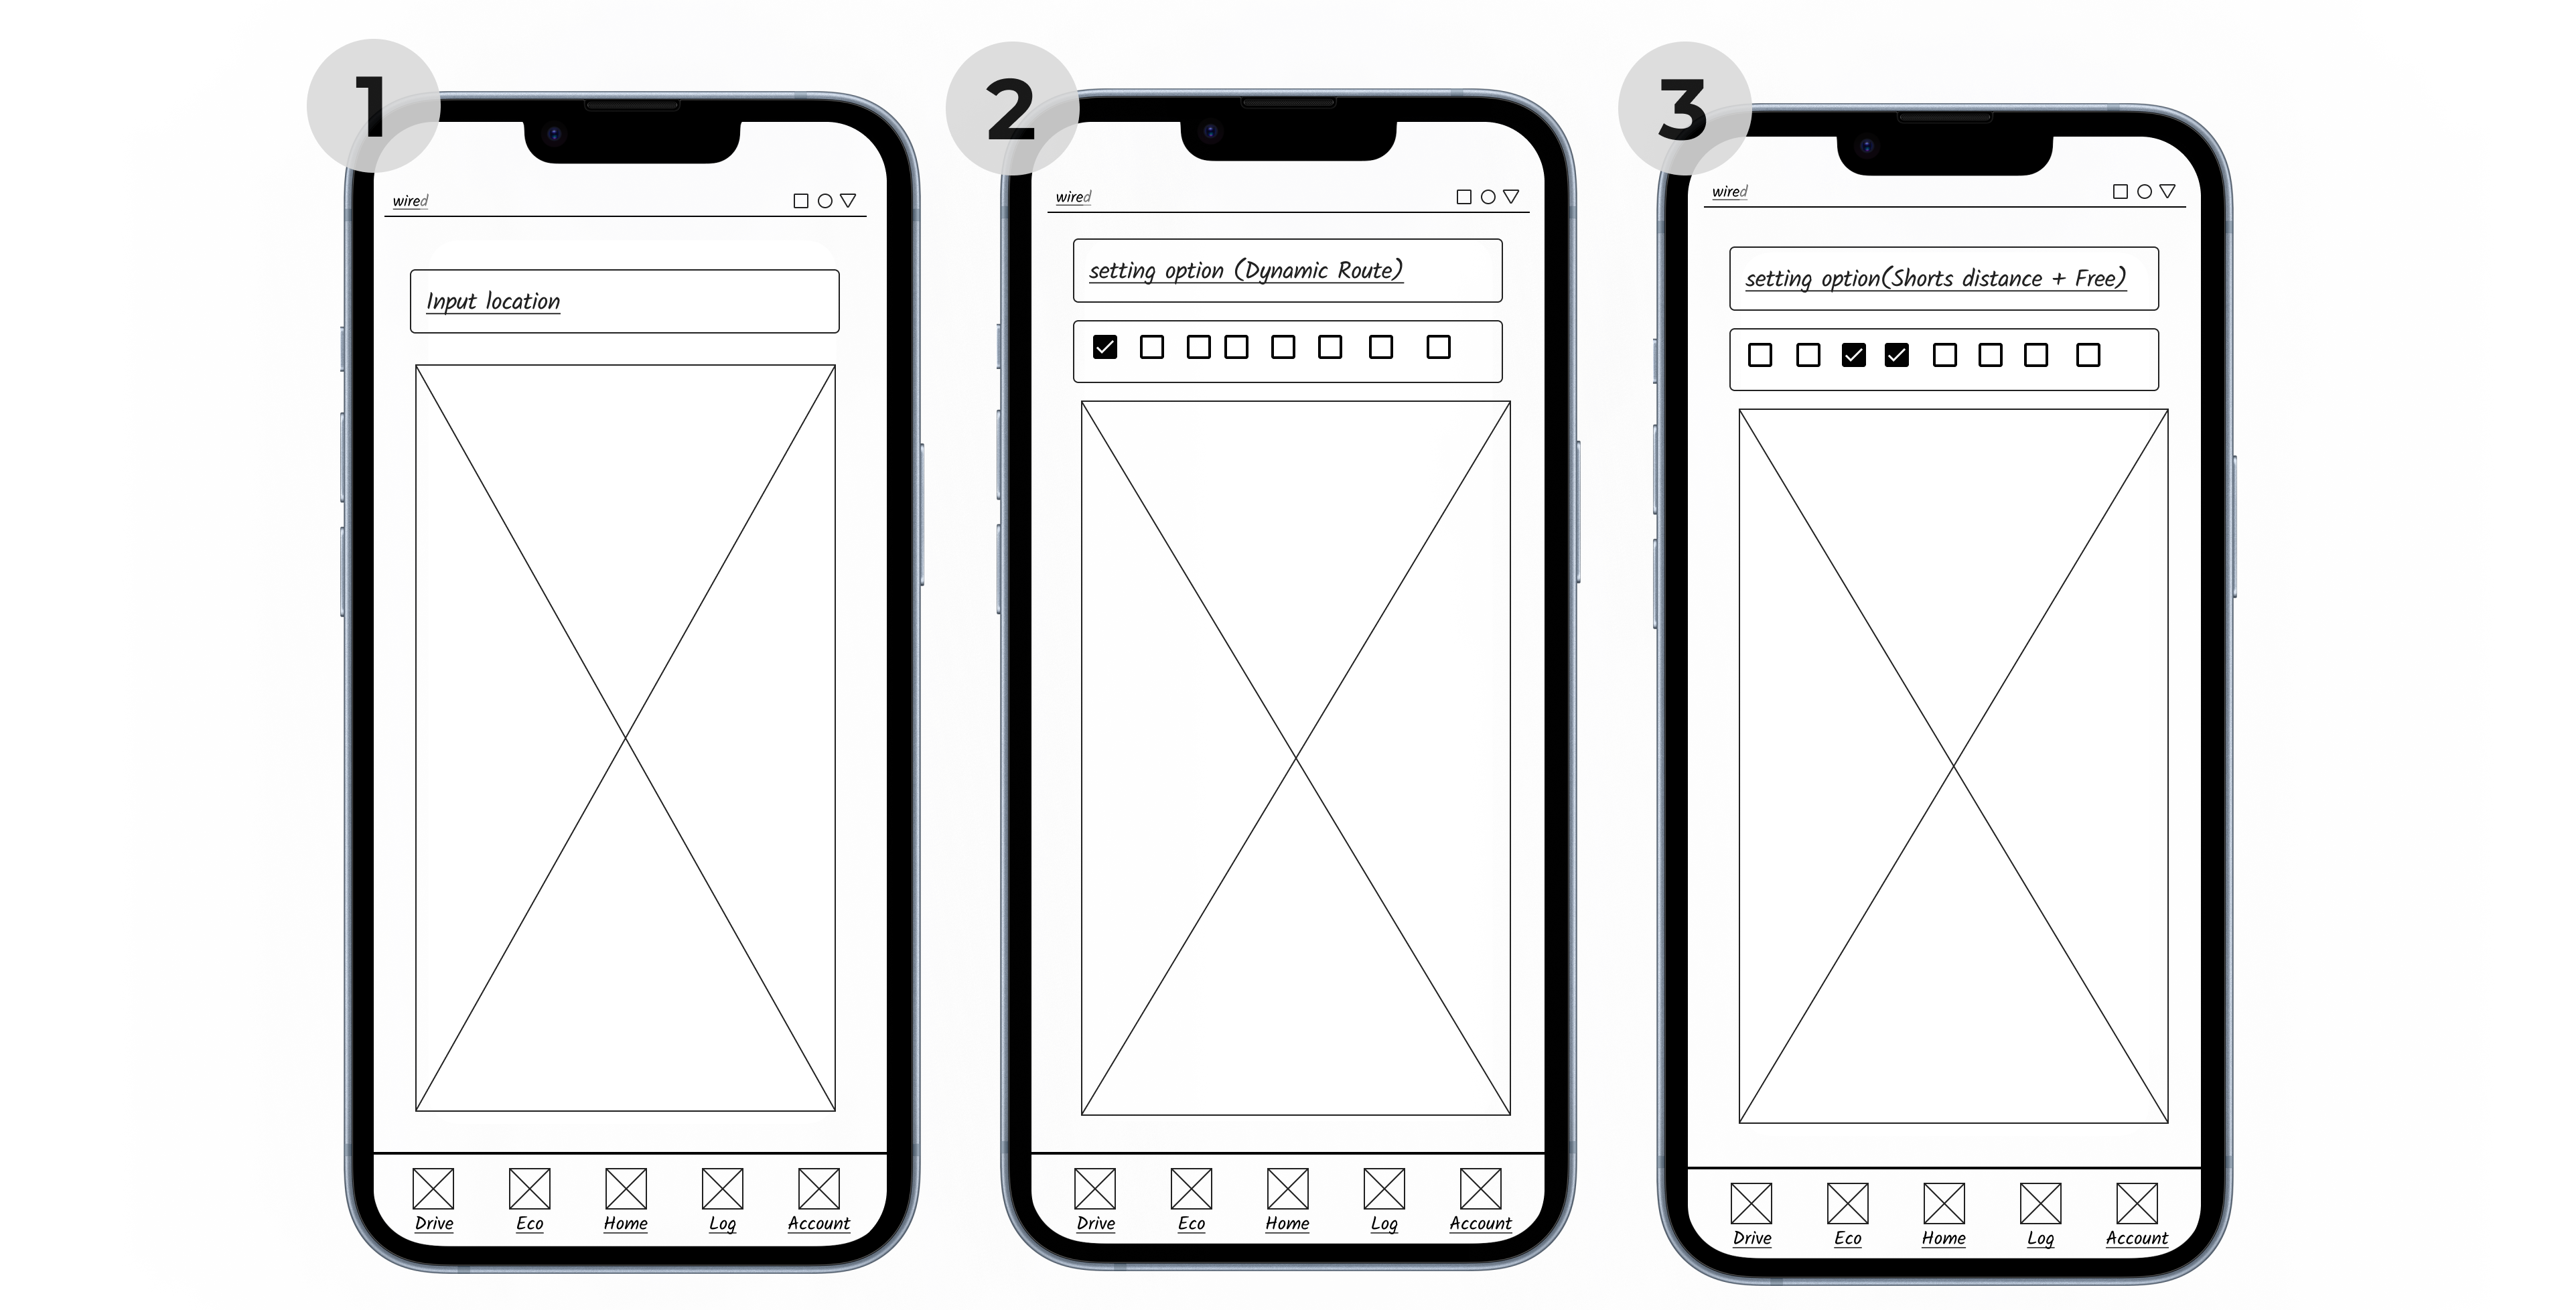
\includegraphics[width=0.8
    \textwidth]{images/Prototype Figures/Prototype Figure 4.png}
    \caption{Dynamic Alternative Route Planner}
    \label{fig:example}
\end{figure}


\noindent In Figure 10, to access premium features, user can upgrade by simply selecting the upgrade button from their current basic plan to a premium plan. Before upgrading, users can view detailed descriptions of the premium plan inclusion. Upon choosing to upgrade, users are directed to payment options and can complete the transaction through our application, integrated with third-party payment providers. After completing the payment, users gain immediate access to the premium services.\\
\begin{figure}[H]
    \centering
    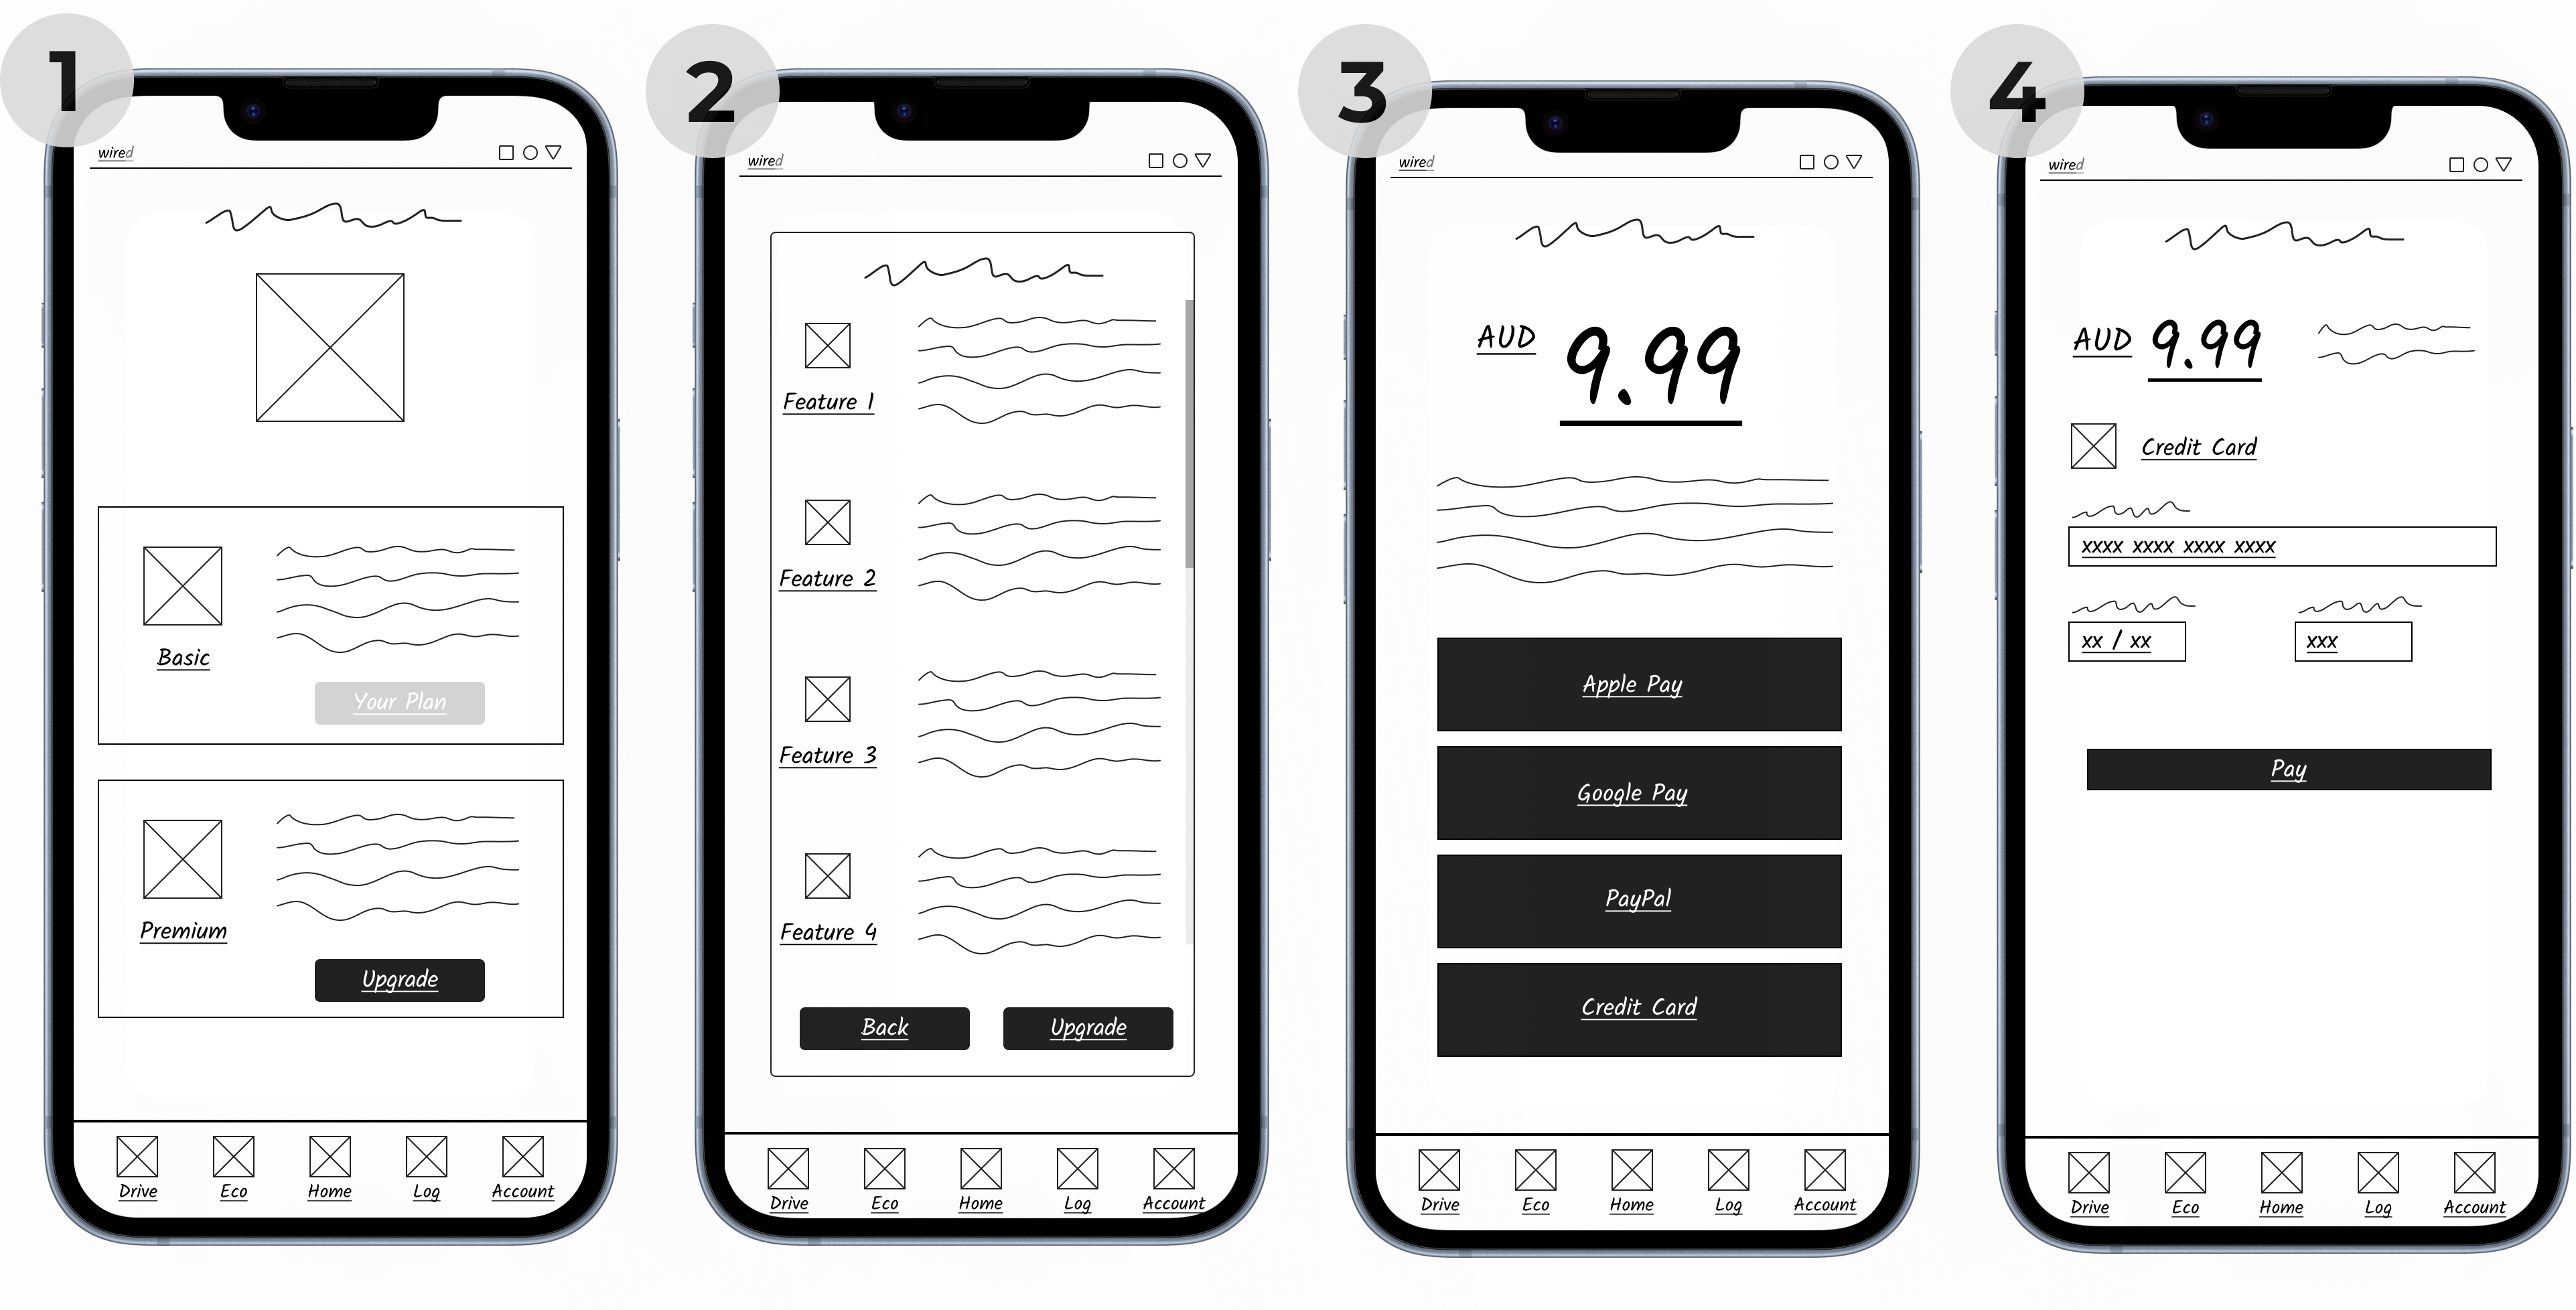
\includegraphics[width=0.8\textwidth]{images/Prototype Figures/Prototype Figure 5.png} 
    \caption{Dynamic Alternative Route Planner}
    \label{fig:routeplanner}
\end{figure}


\noindent In Figure 11, the driving monitor, a premium feature offering advanced services such as real-time road monitoring, driving weather conditions, nearby emergency vehicle locations, and driver behavior monitoring for detecting unsafe practices like sudden hard braking. It utilizes technology and phone sensors to enhance safety and offer rewards for each safely completed journey. Reward points serve as a gamification strategy, encouraging users to earn points redeemable for fuel vouchers as incentives for driving safely.\\
\begin{figure}[h]
    \centering
    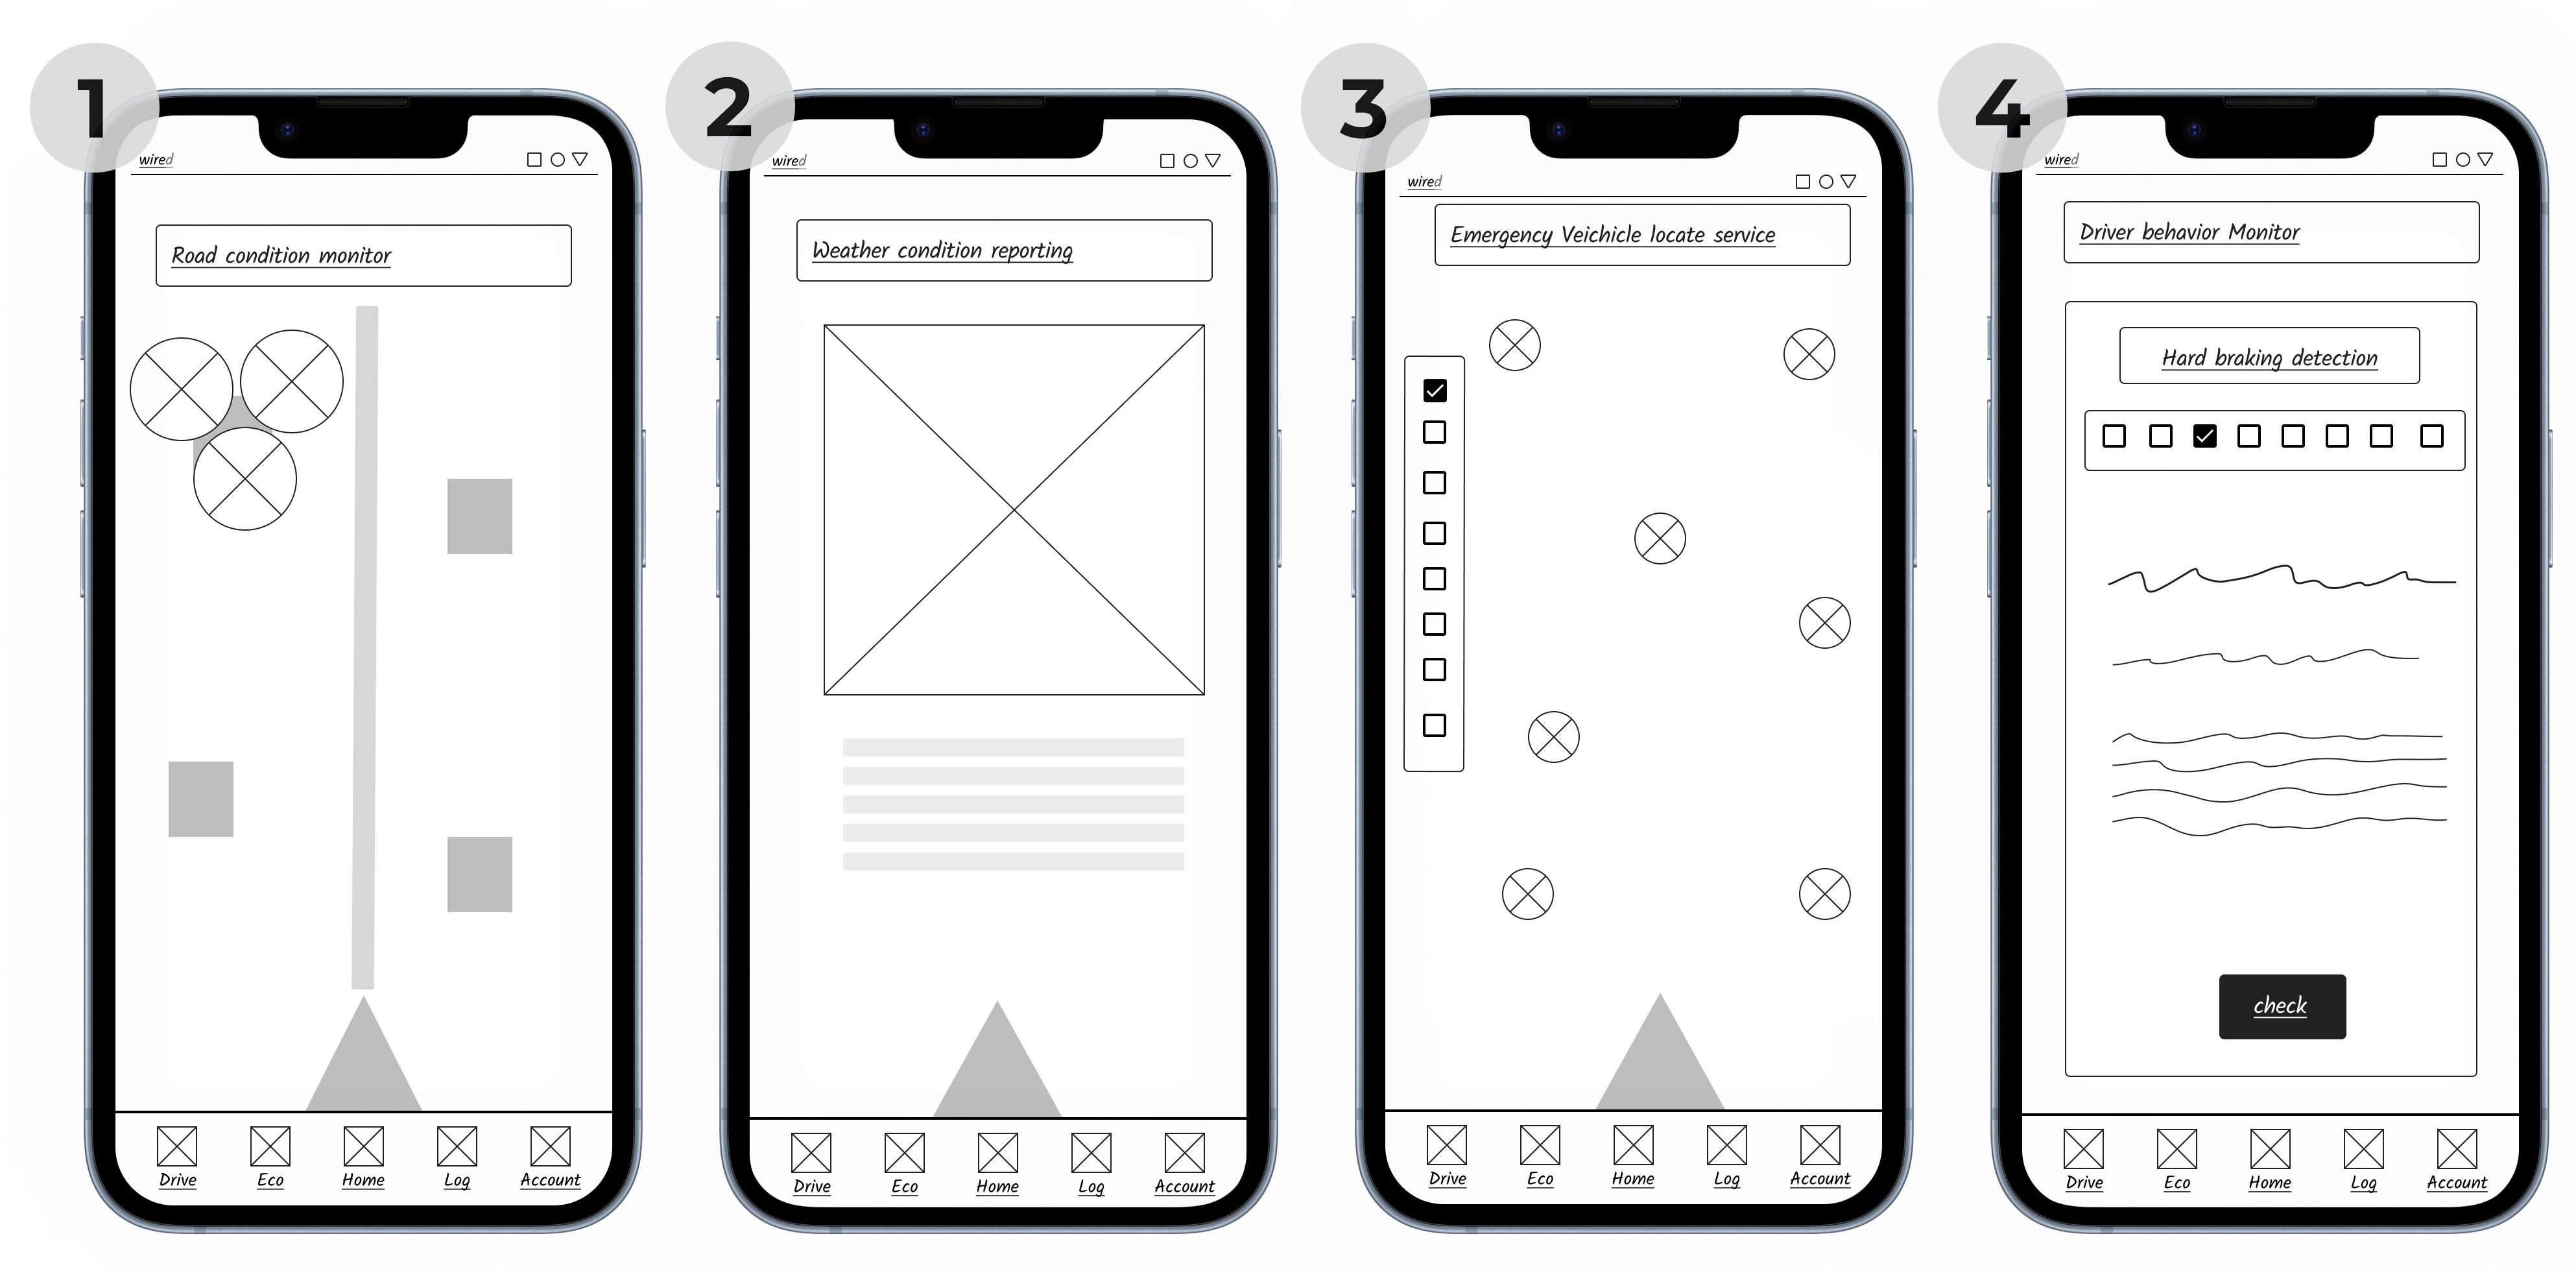
\includegraphics[width=0.8
    \textwidth]{images/Prototype Figures/Prototype Figure 6.png}
    \caption{Driving Monitor}
    \label{fig:example}
\end{figure}




\noindent In Figure 12, another premium feature under the `Log' menu is the vehicle maintenance tracking that allows drivers to maintain a history of vehicle maintenance logs. After subscribing, users must register their vehicle details, including model, year, engine, color, insurance package and company, and ownership details. Some smart cars can also connect directly to the maintenance log. Once set up, users can view all maintenance activities and historical service records on the tracking dashboard.\\

\pagebreak

\begin{figure}[h]
    \centering
    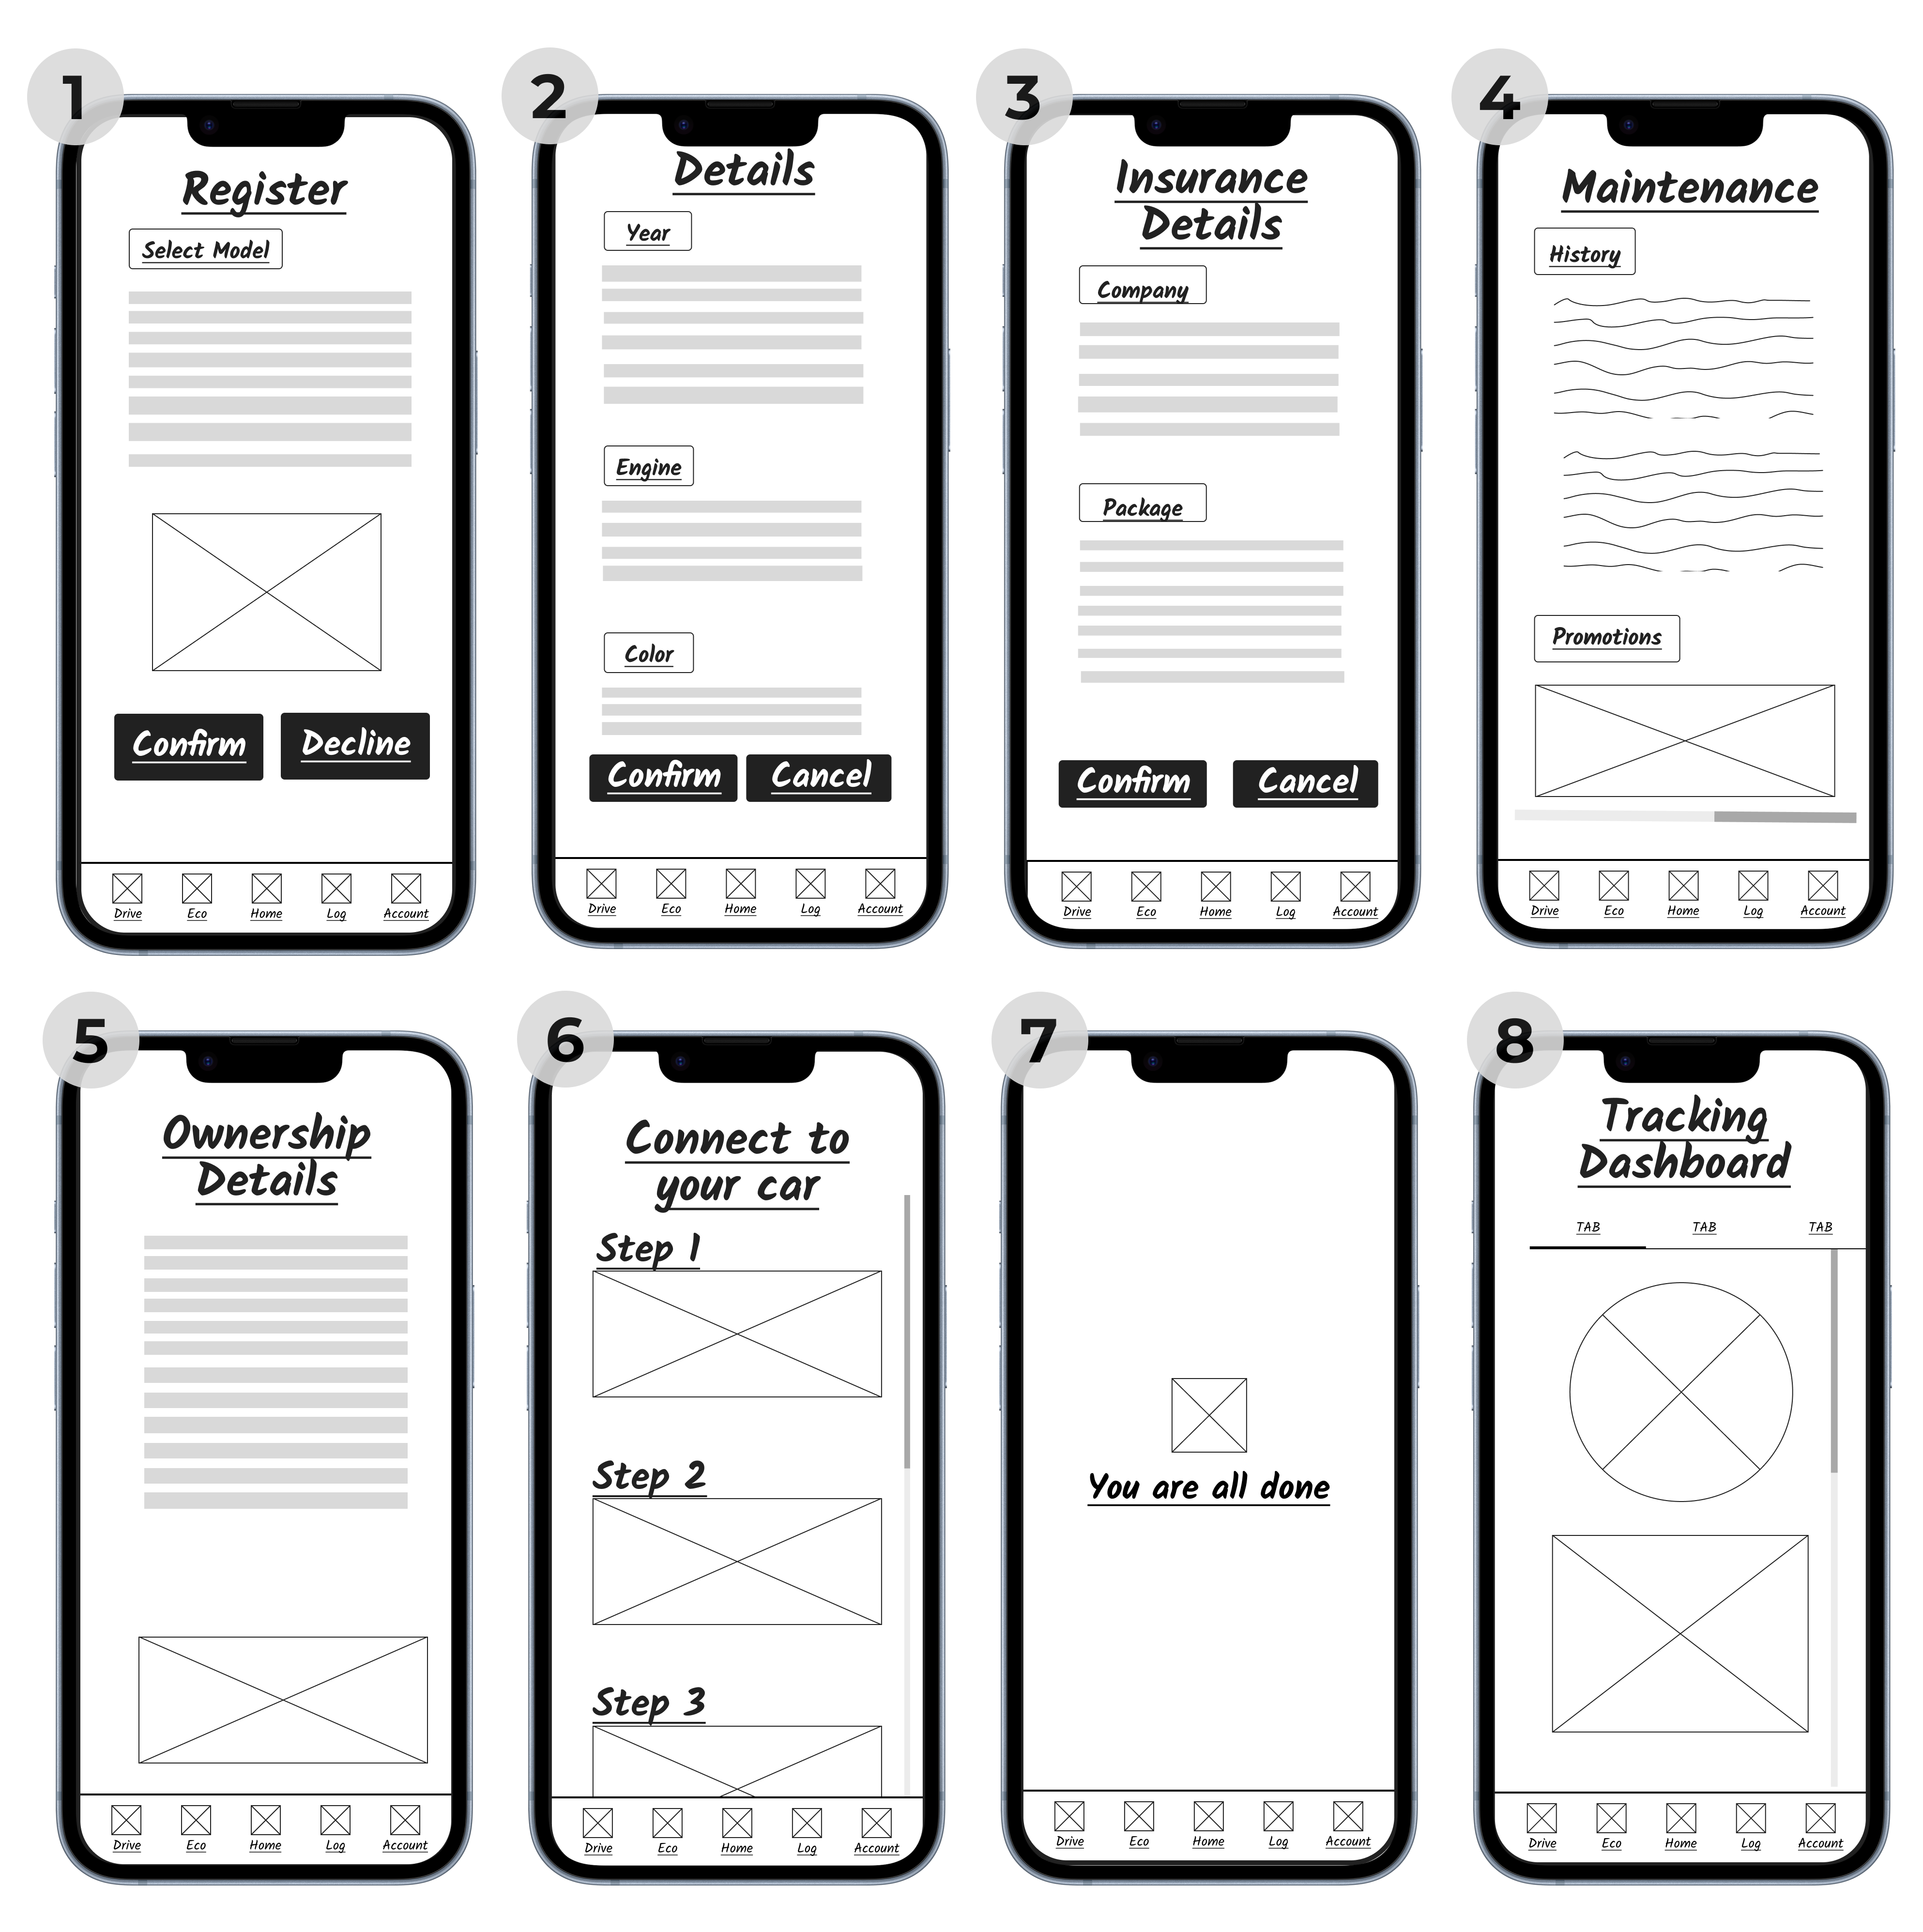
\includegraphics[width=0.8
    \textwidth]{images/Prototype Figures/Prototype Figure 7.png}
    \caption{Vehicle Maintenance Tracking}
    \label{fig:example}
\end{figure}




\noindent The final premium feature is available under the `Account' tab, as shown in Figure 13, that addresses legal penalties that may arise from violations of driving policies. The application connects to a secure government's database for penalty records based on users' driving licenses. Users must first register with official documents and accept all agreement policies. Once finished, they can view each penalty history with details, receive alerts for new penalties, see all fines issued by police authorities, and pay penalties directly on the application based on the provided penalty number. This feature facilitates easier payment of driving penalties.\\
\begin{figure}[h]
    \centering
    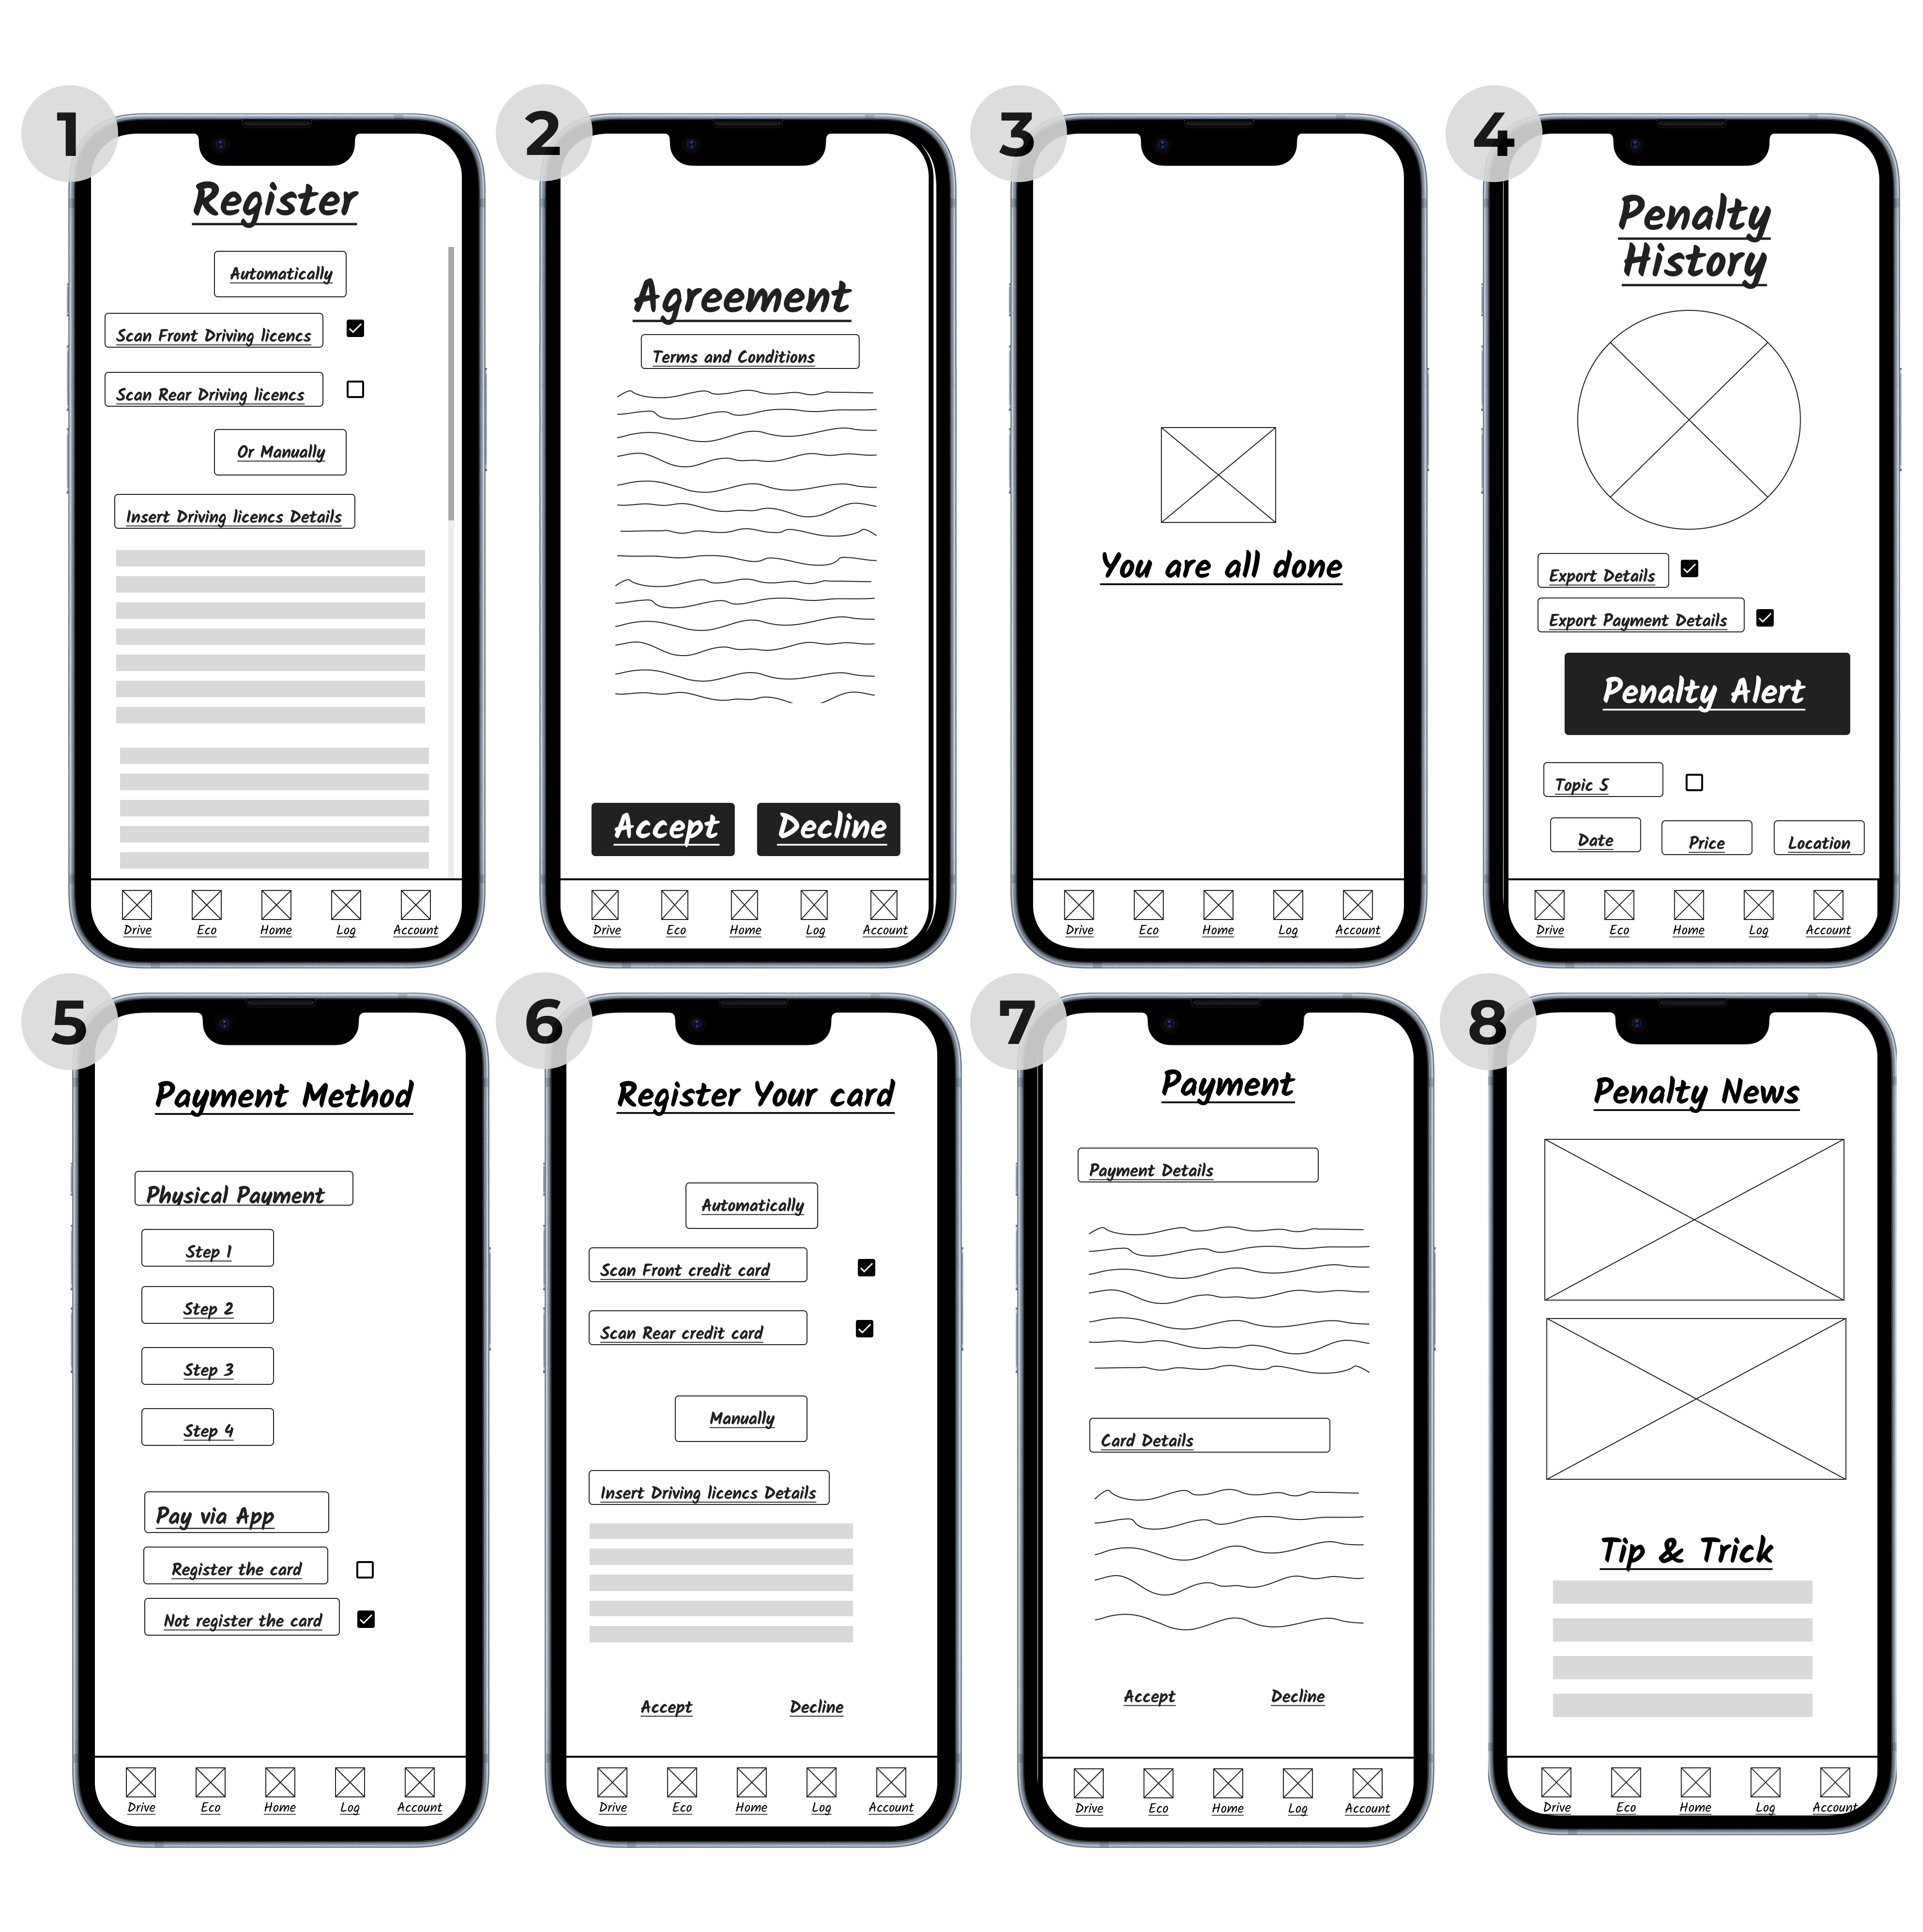
\includegraphics[width=0.8
    \textwidth]{images/Prototype Figures/Prototype Figure 8.png}
    \caption{Recording Penalty History}
    \label{fig:example}
\end{figure}
\pagebreak



\noindent Our prototypes provide a general overview of our screen display, serving as the initial version of our ideation blueprint. As low-fidelity prototypes, they have been validated through research for their usability as a foundational version, aiding in the refinement of high-fidelity prototypes in the final stages \citep{question_6.2}.\\

\pagebreak

%%%%%%%%%%%%%%%%%%%%%%%%%%%%%%%%%%%%%%%%%%%%%%%%%%%%%%%%%%%%%%%%%%%%%%%%%%%%%%%%

\setcounter{page}{17}
\label{sec:Question 7}
\section{Task 7}

\subsection{Future Growth of ClearWay application Recommendations}
\noindent Our application intends to be a leader in the market. We have listed our future outline that will be achieved following below.\\

\noindent \textbf{Analyse customer behaviour and optimise the balance:} \\
\noindent  According to Holm \citep{task_7.1}, the huge amount of resources spent on data analytics creates a successful company. Identifying what is accessible and what is premium is crucial to maintaining competitive advantage \citep{task_7.1}. However, the challenge of freemium is balancing these. To optimise this, customer data must be available. Fortunately, our big customer base allows us to analyse it. We plan to implement this insight to help us create outstanding customer service.\\

\noindent \textbf{Maintain the superior quality:} \\
\noindent  It is necessary to offer value for free and premium users, which is the key to success for freemium, by continuing to improve the value proposition \citep{task_7.1}. According to Holm \citep{task_7.1}, this strategy builds customer relationships, strengthens customer retention, and especially increases switching costs. However, the switching cost is considered low due to the free offering, which means the R\&D department requires sufficient funds to develop new products continuously \citep{task_7.1}. We have adjusted our investment to increase switching costs by creating top-notch services to maintain and attract customers.\\

\noindent \textbf{Social network and collaboration:} \\
\noindent  Our application aims to expand our customer network by using social channels to attract new customers. Moreover, we realise that we must strengthen customer retention, and collaboration is inevitable. Due to our strong business value, we plan to launch marketing campaigns on their channels, such as Facebook, X, and LinkedIn, to reach new customers and enhance the company's reputation. Interestingly, we plan to launch an inviting campaign that invites friends to register for the application and will get incentives like a discount on our partner products and services. \\

\subsection {Benefits \& Value to stakeholders} \\
\noindent \textbf {Growing up customer base:} \\
\noindent  Our superior service continuously expands our lifetime customers and attracts new ones. Moreover, it increases the cost of switching to existing customers and improves the reputation that our partnership relies on to benefit their company. We believe this will convert free users into premium users in the subsequent years.\\

\noindent \textbf {Create a sustainable revenue stream:} \\
\noindent  According to Kumar, in the early 2000s, monthly subscriptions provided a more sustainable revenue stream than advertising \citep{task_7.2}. Investing in superior products increases the premium rate. More importantly, it allows users to use top-notch services, greatly enhancing their experience and improving their safety.\\

\noindent \textbf {Specify the customer need:} \\
\noindent  We have gotten the customers' insight, which we have adopted in our services, directly catching the customer's needs. We believe this will enhance their driving experience and travel route planning.\\

\noindent \textbf {Rapid growth business:} \\
\noindent  Due to our strong partnership from collaboration, we attract investors to invest in our application, increasing funding for our business activities like developing new features and improving in-application customer experience, which will enhance our employee work. For instance, when they have a sufficient budget, they bring into their creativity that creates outstanding services.\\

\noindent \textbf {Easy to reach:} \\
\noindent  Due to collaboration, we will extend our channel to potential users via various channels. From this activity, we expected that this would help our application expand its customer base and help us move closely to what customers need.\\



\pagebreak


% BIBLIOGRAPHY %%%%%%%%%%%%%%%%%%%%%%%%%%%%%%%%%%%%%%%%%%%%%%%%%%%%%%%%%%%%%%%%%%%%%%%%%%%%%%%%%%%% 

% Use Leeds Harvard referencing template
\bibliographystyle{lsharvard}
% Add here the bib file with your references
\bibliography{references}
	
\def\UrlBreaks{\do\/\do-}

\clearpage



\setcounter{page}{21}
\textbf{Appendix : Group Members' Contribution Table}\\
\begin{figure}[h]
    \centering
    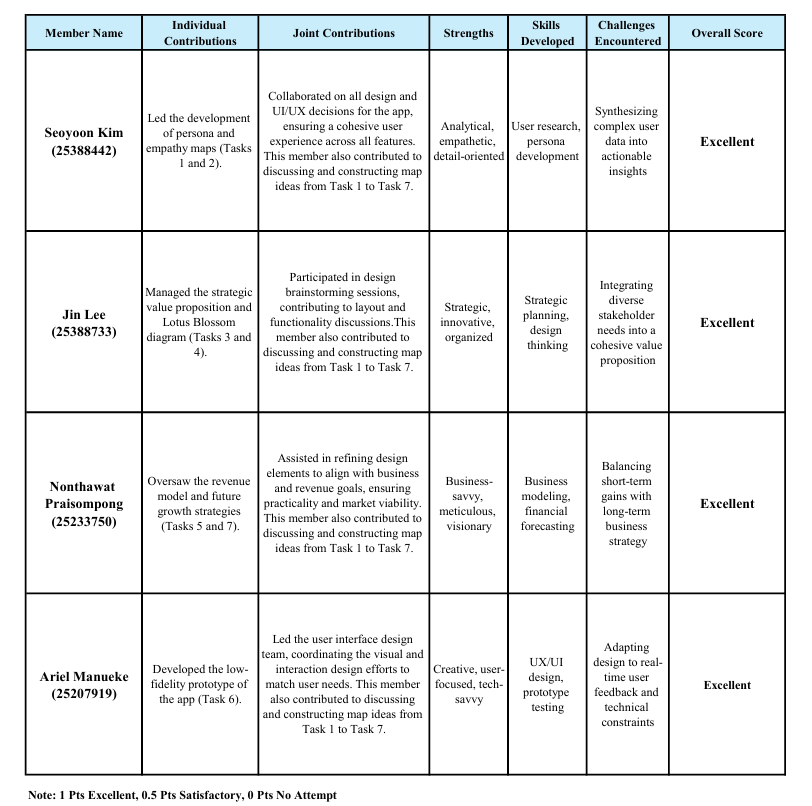
\includegraphics[width=1.0
    \textwidth]{images/Group members.png}
\end{figure}



\end{document}


%%%%%%%%%%%%%%%%%%%%%%%%%%%%%%%%%%%%%%%%%%%%%%%%%%%%%%%%%%%%%%%%%%%%%%%%%%%%%%%%%%%% 

